\chapter{Software Requirement Specifications}
\label{ch:srs}

This chapter specifies what KhetLens must do and how well. It lists the features, the functional and non-functional requirements, the assumptions, the use cases in the department's tabular format, the hardware and software needed, the user interface, the database design and the risks. Requirement identifiers (F, FR, NFR, UC, R) are used in the following chapters and will be the basis of the traceability matrix in the implementation report.

\section{List of Features}
\label{sec:features}
\begin{description}[style=nextline, leftmargin=0pt, itemsep=2pt]
  \item[F1 Offline plant-photo diagnosis.] Identify the crop and one of 17 conditions from a photograph of the plant, close up or from a short distance, on the device.
  \item[F2 Capture with live quality feedback.] Real-time blur and exposure warnings before the shutter is pressed, and a quality check after it.
  \item[F3 Weather-aware result.] Adjust the image result using the recent weather of the farmer's district.
  \item[F4 Three-state outcome.] Every diagnosis ends as \emph{Confident}, \emph{Likely} (follow-up questions) or \emph{Unsure} (no guess).
  \item[F5 Picture-based follow-up questions.] Up to three questions, answered by tapping illustrated options.
  \item[F6 Explained result.] Each result shows the reasons behind it and lets the farmer correct the detected crop.
  \item[F7 Treatment guidance.] Treatment and prevention steps per condition, with source and reviewer shown, in three languages with audio.
  \item[F8 Offline disease library.] Reference for all 17 conditions: symptoms, causes, management, audio.
  \item[F9 Diagnosis history.] Diagnoses stored automatically and kept for six months.
  \item[F10 Farmer feedback.] Correctness and treatment-outcome feedback, captured offline, sent when connected and then removed from the phone.
  \item[F11 Three-language interface with audio.] English, Urdu and Punjabi text with recorded audio on every content screen.
  \item[F12 Sign-in with guest mode.] Phone-number sign-in with a one-time code over WhatsApp; diagnosis never requires an account.
  \item[F13 Background updates.] Weather refresh, feedback upload and model or content updates whenever the phone is connected.
\end{description}

\section{Functional Requirements}
\label{sec:fr}
\subsection{Onboarding and account}
\begin{itemize}
  \item \textbf{FR-01} On first launch the system shall offer English, Urdu and Punjabi, each with an audio button that speaks the language name; the choice shall be changeable in Settings. (Farmer)
  \item \textbf{FR-02} The system shall allow sign-in by mobile number: it sends a one-time code over WhatsApp, verifies it, and keeps the farmer signed in while offline. (Farmer)
  \item \textbf{FR-03} The system shall offer ``Skip for now''; in guest mode all diagnosis, library and history functions work, and only feedback upload waits for sign-in. (Farmer)
  \item \textbf{FR-04} The system shall request location permission once, derive the farmer's district on the device, display it, and allow it to be changed manually. (Farmer)
\end{itemize}
\subsection{Capture and diagnosis}
\begin{itemize}
  \item \textbf{FR-05} The system shall provide a camera screen with brief guidance and shall also accept an image from the gallery. (Farmer)
  \item \textbf{FR-06} While the viewfinder is open the system shall show a live warning when the preview is blurred or badly exposed. (Farmer)
  \item \textbf{FR-07} After capture the system shall check the photograph for blur and exposure; if it fails, the system shall show the reason and ask for a retake without running the classifier. (System)
  \item \textbf{FR-08} The system shall identify the crop and show it on the result screen with a one-tap correction; if crop confidence is low it shall ask the farmer to confirm the crop first. (System, Farmer)
  \item \textbf{FR-09} The system shall classify the photograph into one of the conditions of the detected crop, on the device and without network access, whether it is a close-up of a leaf or a wider shot of the plant; wider shots are analysed as a whole and in regions, and the results combined. (System)
  \item \textbf{FR-10} The system shall adjust the class probabilities using the stored weather of the district when a recent snapshot exists; otherwise it shall use the image result alone and say so. (System)
  \item \textbf{FR-11} The system shall compute a novelty score and a calibrated confidence for every diagnosis and assign one of three outcomes: Confident, Likely or Unsure. (System)
  \item \textbf{FR-12} For a Confident outcome the system shall show the condition name, the confidence, a ``Disease confirmed'' or ``Healthy'' badge and at least two reasons. (System)
  \item \textbf{FR-13} For a Likely outcome the system shall ask up to three picture-based questions from the crop's question set and finalise as Confident or Unsure; ``Not sure'' shall be an option for every question. (Farmer)
  \item \textbf{FR-14} For an Unsure outcome the system shall state that nothing was guessed, give the reason, offer to take two more photographs, and offer a field-officer contact; no treatment shall be shown. (System)
\end{itemize}
\subsection{Guidance, library and audio}
\begin{itemize}
  \item \textbf{FR-15} For a Confident result the system shall show treatment and prevention guidance with a safety note, the source and the reviewing agronomist, in the selected language. (Farmer)
  \item \textbf{FR-16} Guidance shall name approved product types and refer to label doses; specific doses appear only where approved by the reviewer. (Content)
  \item \textbf{FR-17} The system shall provide a library of all 17 conditions, filterable by crop, each with symptoms, causes, management and audio, fully offline. (Farmer)
  \item \textbf{FR-18} Every content screen shall have a speaker button that plays recorded audio in the selected language. (Farmer)
\end{itemize}
\subsection{History and feedback}
\begin{itemize}
  \item \textbf{FR-19} The system shall store every completed diagnosis automatically with its photograph, result, confidence and weather snapshot, and shall clear entries older than six months. (System)
  \item \textbf{FR-20} The system shall list recent diagnoses and open any of them to show the full result and guidance. (Farmer)
  \item \textbf{FR-21} The system shall let the farmer record whether a diagnosis was correct and whether the treatment worked, with an optional comment, store it locally and queue it for upload. (Farmer)
  \item \textbf{FR-22} Sharing a photograph with feedback shall be an explicit opt-in; by default photographs do not leave the device. (Farmer)
\end{itemize}
\subsection{Connectivity, updates and backend}
\begin{itemize}
  \item \textbf{FR-23} When connected, the system shall fetch the recent weather (daily temperature, humidity and rainfall over the last two weeks) for the district and store it; the home screen shall show a summary and its age. (System)
  \item \textbf{FR-24} When connected, the system shall upload queued feedback, delete the local copy once the server acknowledges it, and retry later on failure. (System)
  \item \textbf{FR-25} When connected, the system shall check for a newer model or content pack, download it in the background, verify it and switch to it; a failed download shall leave the current version in use. (System)
  \item \textbf{FR-26} The application package shall include a baseline model and content pack so that every function works on first launch. (System)
  \item \textbf{FR-27} The server shall provide endpoints for code request and verification, feedback ingestion, and model and content distribution, and shall store feedback without the farmer's name. (Server)
  \item \textbf{FR-28} The team shall publish new content or models through a tool that validates the content, checks that every guidance entry has a source and reviewer, and records the version. (Team)
\end{itemize}

\section{Quality Attributes}
\label{sec:qa}
In order of priority: \textbf{availability offline} (every farmer-facing function works with no network); \textbf{performance on entry-level hardware}; \textbf{trustworthiness} (calibrated confidence, honest abstention, explained results, attributed guidance); \textbf{usability for low-literacy users} (icon-first, one-handed, audio everywhere, large type, high contrast); \textbf{privacy} (photographs and precise location stay on the device unless shared deliberately); \textbf{maintainability} (model and content updatable without a release); and \textbf{robustness} (sensible behaviour on missing weather, failed downloads and interrupted connectivity).

\section{Non-Functional Requirements}
\label{sec:nfr}
{\small
\begin{longtable}{|L{1.3cm}|L{2.4cm}|L{7.5cm}|L{3.0cm}|}
\caption{Non-functional requirements.}\label{tab:nfr}\\
\hline
\textbf{ID} & \textbf{Category} & \textbf{Requirement} & \textbf{Verification} \\ \hline
\endfirsthead
\multicolumn{4}{l}{\small\textit{Table \thetable\ continued}}\\ \hline
\textbf{ID} & \textbf{Category} & \textbf{Requirement} & \textbf{Verification} \\ \hline
\endhead
\hline \multicolumn{4}{r}{\small\textit{continued on next page}}\\
\endfoot
\endlastfoot
NFR-01 & Performance & A diagnosis is returned within about two seconds on an entry-level Android phone using the CPU only; app start-up within a few seconds. & Measurement on target phones \\ \hline
NFR-02 & Resource use & Model under 10\,MB; content pack with audio under 60\,MB; total install under 150\,MB. & Build artefacts \\ \hline
NFR-03 & Availability & All farmer-facing use cases pass with the network disabled. & Test cases in airplane mode \\ \hline
NFR-04 & Accuracy & Accuracy and macro-F1 reported on a held-out set of field photographs for every model release, with a release target of macro-F1 of 0.80 or higher. & Evaluation report \\ \hline
NFR-05 & Trustworthiness & Calibration error kept low through temperature scaling; unsupported inputs rejected at a high rate while keeping accuracy on supported classes; blurred photographs reliably sent for retake. & Evaluation report \\ \hline
NFR-06 & Usability & Home to treatment in at most four taps; tap targets of at least 48\,dp; body text of at least 16\,sp; checked with farmers through our partner. & UI audit; farmer test \\ \hline
NFR-07 & Localisation & All strings, library entries and guidance available in the three languages, with correct right-to-left layout and Nastaliq rendering and audio on every content screen. & Content audit \\ \hline
NFR-08 & Privacy & Photographs and GPS coordinates never sent without opt-in; only the district stored on the server; sign-in tokens stored in encrypted storage; all traffic over TLS. & Code review \\ \hline
NFR-09 & Reliability & No data loss if the app is closed during a diagnosis or feedback entry; a failed update never leaves the app without a working model. & Fault-injection tests \\ \hline
NFR-10 & Compatibility & Android 8.1 and later; no dependency on a GPU or neural accelerator for core functions. & Device tests \\ \hline
\end{longtable}
}

\section{Assumptions}
\label{sec:assumptions}
\begin{itemize}
  \item Farmers have access to an Android phone meeting NFR-10 with a working camera and about 1\,GB of free storage.
  \item Phones connect to a network at least occasionally, which is enough for weather refresh, feedback upload and updates.
  \item Farmers who sign in have WhatsApp on the same number; those who do not can use guest mode.
  \item Our partner's agronomists review the disease list, treatment content and follow-up questions, and field officers support photograph collection during the growing seasons.
  \item Public datasets are used under their published terms; each source's licence is recorded when it is added.
  \item A free weather service is sufficient for the request volumes involved; the weather module is isolated so another provider can be substituted.
  \item Treatment content is advisory; the farmer and the agronomist remain responsible for product selection and dosing.
\end{itemize}

\section{Use Cases}
\label{sec:usecases}
Figure~\ref{fig:usecase} shows the use-case model. UC-01 to UC-12 belong to the farmer, UC-13 and UC-14 are system-initiated, and UC-15 and UC-16 belong to the team and the agronomist. Each is specified below in the department's format.

\begin{figure}[H]
  \centering
  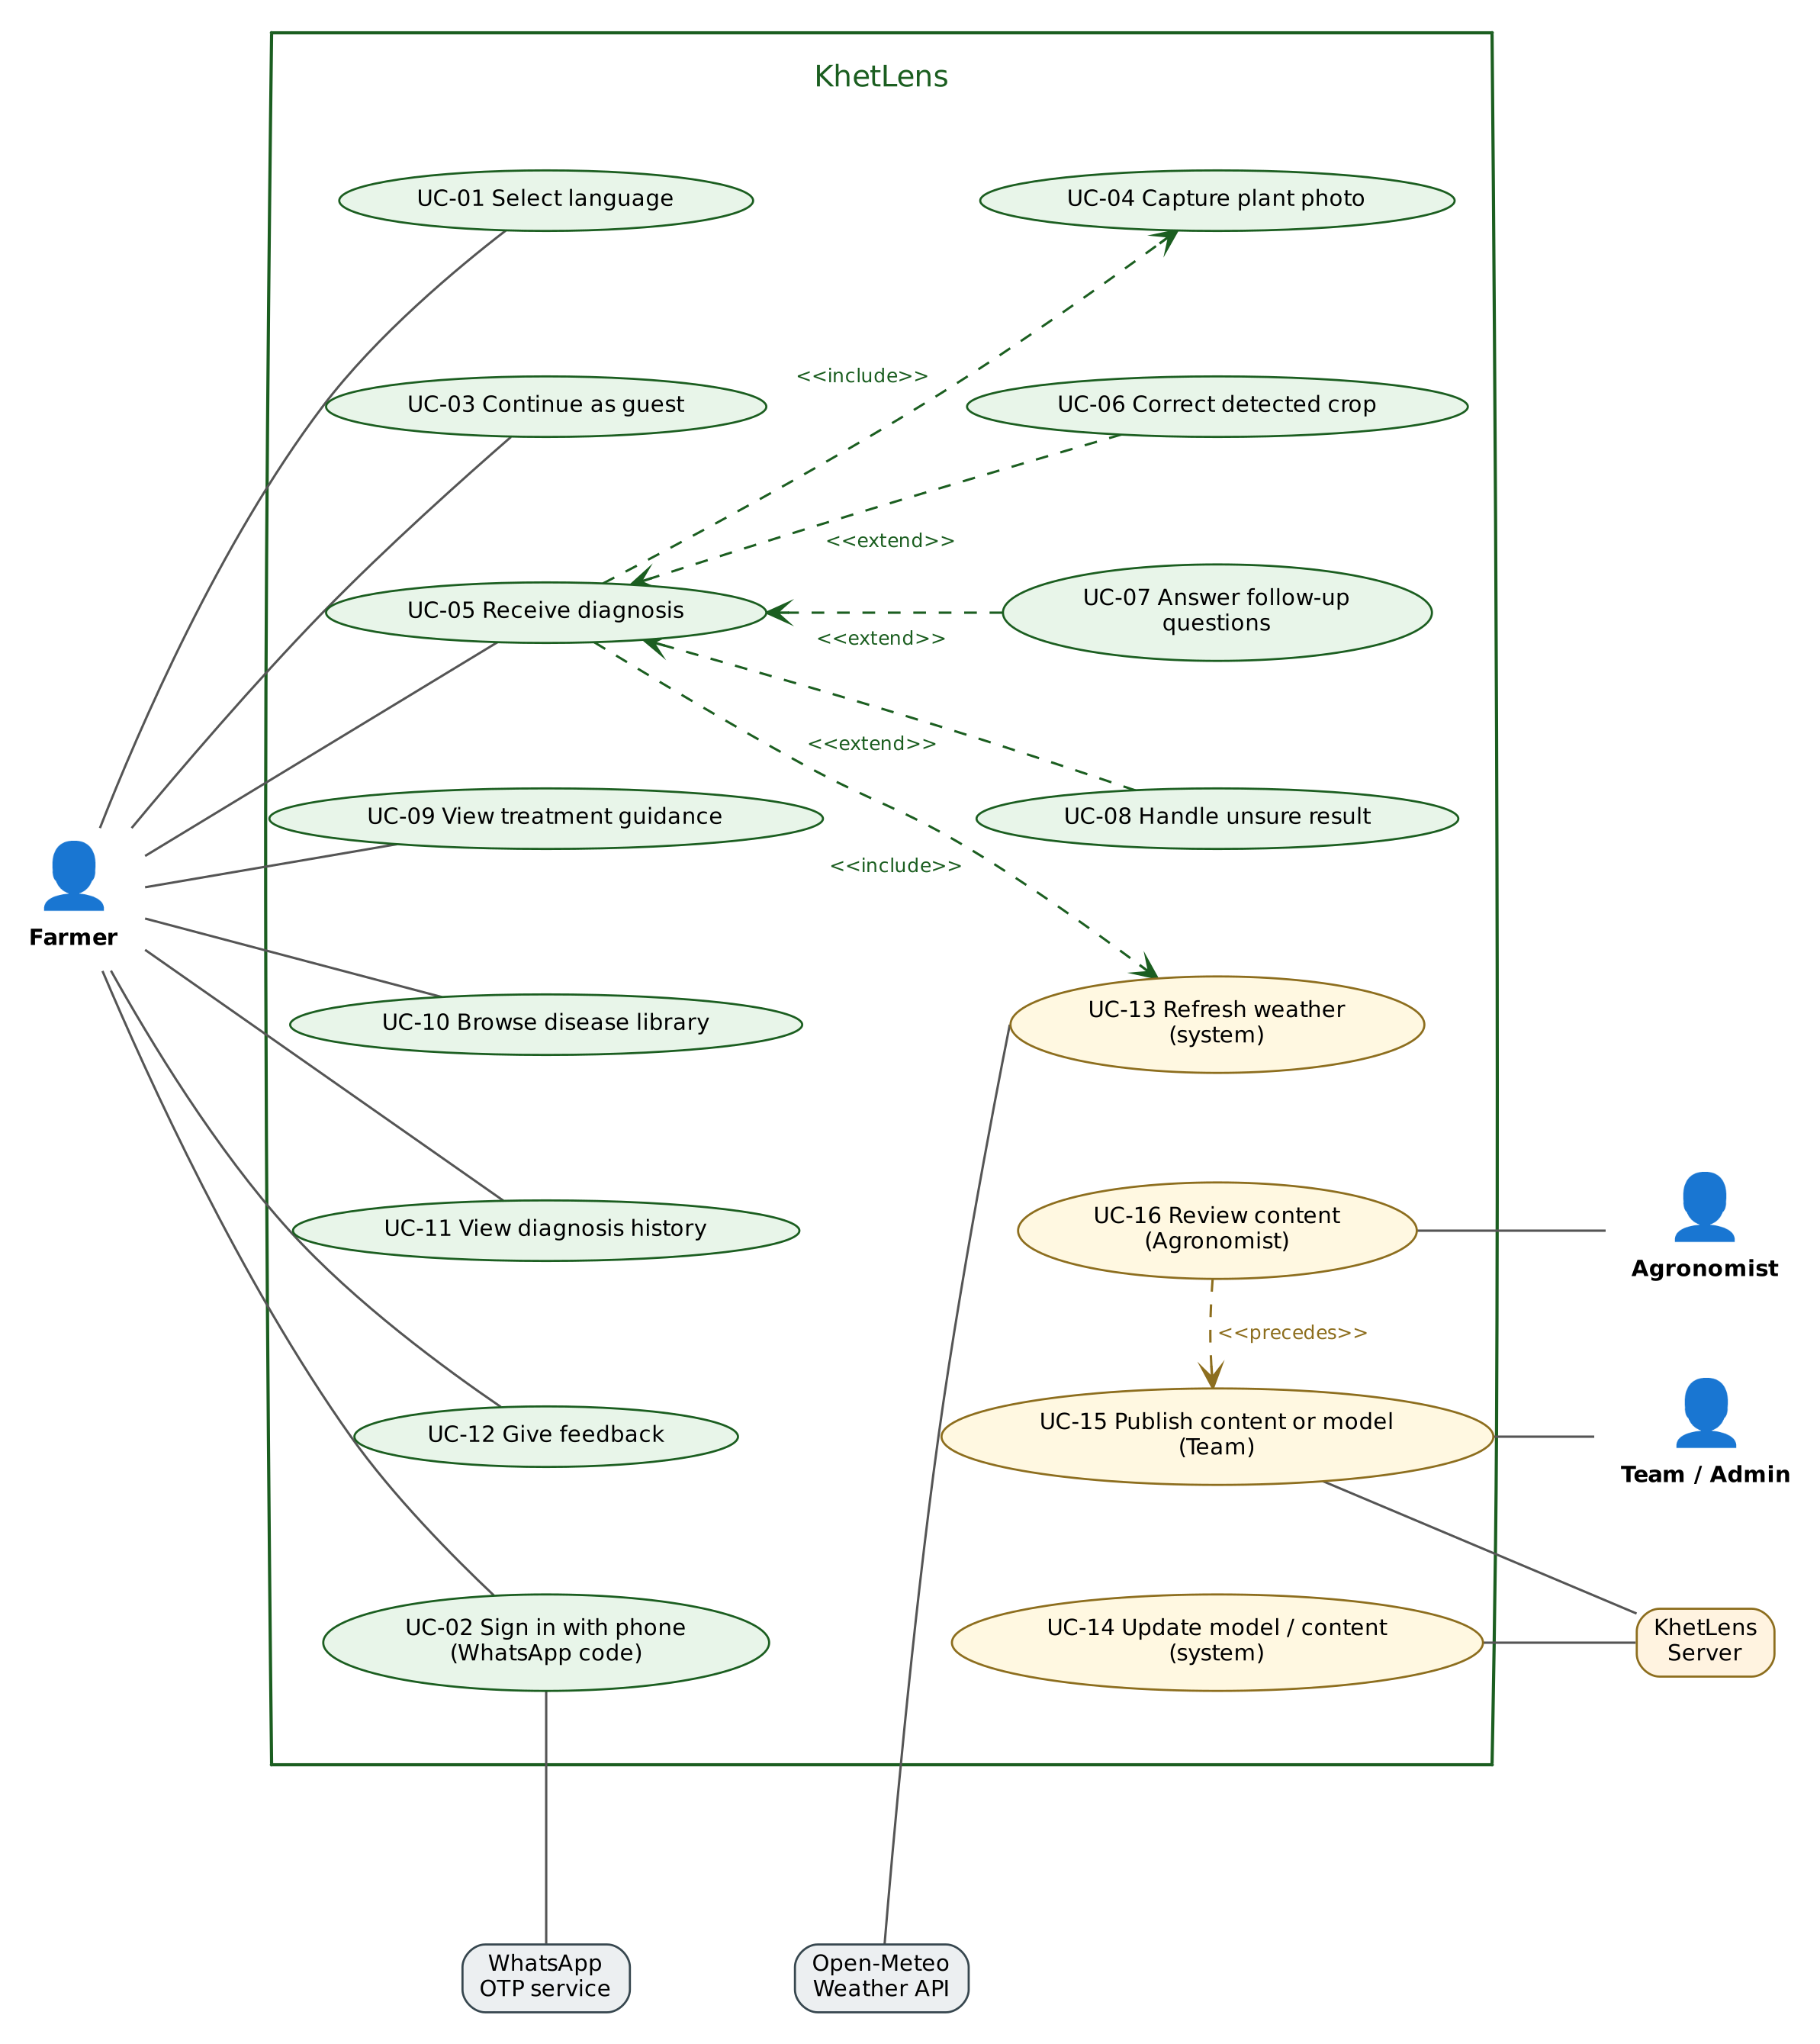
\includegraphics[width=\textwidth,height=0.88\textheight,keepaspectratio]{Figures/diagrams/usecase.png}
  \caption{Use-case diagram of KhetLens.}
  \label{fig:usecase}
\end{figure}

\begin{usecase}{UC-01 Select language}{uc:01}
\ucrow{Name}{Select language}
\ucrow{Actors}{Farmer}
\ucrow{Summary}{The farmer chooses English, Urdu or Punjabi on first launch or from Settings; the interface, library and audio switch to that language.}
\ucrow{Pre-Conditions}{Application installed and opened.}
\ucrow{Post-Conditions}{Language preference saved; all screens rendered in that language.}
\ucrow{Special Requirements}{Each option has a speaker button so that a non-reader can choose.}
\ucflow{Basic Flow}
\ucstep{1. Farmer opens the app for the first time.}{2. System shows three language tiles with speaker icons.}
\ucstep{3. Farmer taps a tile and Continue.}{4. System saves the preference and opens the sign-in screen.}
\ucflow{Alternative Flow}
\ucstep{1a. Farmer opens Settings later and taps Language.}{2a. System shows the same tiles and re-renders the current screen on selection.}
\ucstep{3a. Farmer taps a speaker icon first.}{4a. System plays the language name aloud and waits.}
\end{usecase}

\begin{usecase}{UC-02 Sign in with phone (WhatsApp code)}{uc:02}
\ucrow{Name}{Sign in with phone number}
\ucrow{Actors}{Farmer; WhatsApp OTP service}
\ucrow{Summary}{The farmer enters a mobile number, receives a one-time code on WhatsApp, enters it and stays signed in.}
\ucrow{Pre-Conditions}{Phone connected to a network; language selected.}
\ucrow{Post-Conditions}{Sign-in token stored; feedback upload enabled.}
\ucrow{Special Requirements}{Code requests limited per number; sign-in is optional (UC-03).}
\ucflow{Basic Flow}
\ucstep{1. Farmer enters the mobile number and taps Send code on WhatsApp.}{2. System asks the server to send a code and shows the code entry field.}
\ucstep{3. Farmer enters the 6-digit code.}{4. System verifies it with the server, stores the token and opens Home.}
\ucflow{Alternative Flow}
\ucstep{1a. Farmer is offline.}{2a. System explains that sign-in needs a connection and offers Skip for now.}
\ucstep{3a. Farmer enters a wrong or expired code.}{4a. System shows an error and offers to resend after a short wait.}
\end{usecase}

\begin{usecase}{UC-03 Continue as guest}{uc:03}
\ucrow{Name}{Continue as guest}
\ucrow{Actors}{Farmer}
\ucrow{Summary}{The farmer skips sign-in and uses all diagnostic functions without an account.}
\ucrow{Pre-Conditions}{Language selected.}
\ucrow{Post-Conditions}{Guest profile created; feedback is stored but not uploaded until sign-in.}
\ucrow{Special Requirements}{The sign-in prompt is shown only when the farmer tries to send feedback.}
\ucflow{Basic Flow}
\ucstep{1. Farmer taps ``Skip for now''.}{2. System creates a guest profile and opens Home.}
\ucflow{Alternative Flow}
\ucstep{1a. Guest later taps Send feedback.}{2a. System saves the feedback locally and offers sign-in to enable upload.}
\end{usecase}

\begin{usecase}{UC-04 Capture plant photo}{uc:04}
\ucrow{Name}{Capture plant photo}
\ucrow{Actors}{Farmer}
\ucrow{Summary}{The farmer photographs the affected plant, close up or from a short distance, with live blur and exposure feedback; the photograph is quality-checked before diagnosis.}
\ucrow{Pre-Conditions}{Camera permission granted; Home screen open.}
\ucrow{Post-Conditions}{A photograph that passed the check is handed to UC-05; otherwise the farmer is asked to retake.}
\ucrow{Special Requirements}{Live indicator updates smoothly; the quality check adds no noticeable delay.}
\ucflow{Basic Flow}
\ucstep{1. Farmer taps ``Diagnose a plant''.}{2. System opens the camera with the guidance ``Point at the affected plant, hold steady''.}
\ucstep{3. Farmer points the camera at the plant or at a leaf.}{4. System shows a live indicator: green when sharp and well lit, amber when blurred or dark.}
\ucstep{5. Farmer presses the shutter.}{6. System checks blur and exposure and, on pass, continues to UC-05.}
\ucflow{Alternative Flow}
\ucstep{5a. Farmer taps Gallery and picks an image.}{6a. System runs the same check on the chosen image.}
\ucstep{5b. Farmer's photograph is blurred or dark.}{6b. System shows the reason (too blurry, too dark) and returns to the viewfinder.}
\end{usecase}

\begin{usecase}{UC-05 Receive diagnosis}{uc:05}
\ucrow{Name}{Receive diagnosis}
\ucrow{Actors}{Farmer}
\ucrow{Summary}{The system identifies the crop and condition on the device, applies the weather adjustment and the uncertainty check, and shows a Confident, Likely or Unsure outcome.}
\ucrow{Pre-Conditions}{Photograph passed the quality check; model loaded.}
\ucrow{Post-Conditions}{Diagnosis saved in history with outcome, probabilities and weather snapshot.}
\ucrow{Special Requirements}{No network access; uses the stored weather if it is recent (FR-10).}
\ucflow{Basic Flow}
\ucstep{1. Farmer waits after pressing the shutter.}{2. System runs the model: crop head, then the disease head of the detected crop.}
\ucstep{3. Farmer sees the progress indicator.}{4. System computes novelty and confidence, applies the weather prior and assigns the outcome.}
\ucstep{5. Farmer views the result screen.}{6. System shows crop, condition, confidence, badge, the ``Not [crop]?'' chip and the Why panel, and saves the record.}
\ucstep{7. Farmer taps ``See treatment''.}{8. System opens UC-09.}
\ucflow{Alternative Flow}
\ucstep{5a. Farmer sees a crop-confirmation prompt (crop confidence low).}{6a. System shows three crop tiles and continues with the chosen crop (UC-06).}
\ucstep{5b. Farmer sees a Likely result.}{6b. System opens the follow-up questions (UC-07).}
\ucstep{5c. Farmer sees an Unsure result.}{6c. System opens the unsure screen (UC-08).}
\ucstep{5d. Farmer diagnoses with no recent weather stored.}{6d. System uses the image result alone and notes ``Weather context unavailable''.}
\end{usecase}

\begin{usecase}{UC-06 Correct detected crop}{uc:06}
\ucrow{Name}{Correct detected crop}
\ucrow{Actors}{Farmer}
\ucrow{Summary}{The farmer overrides the detected crop; the system re-runs the disease head for the chosen crop.}
\ucrow{Pre-Conditions}{A result is shown, or the system has asked for crop confirmation.}
\ucrow{Post-Conditions}{Record updated with the corrected crop and a correction flag.}
\ucrow{Special Requirements}{Re-inference is immediate.}
\ucflow{Basic Flow}
\ucstep{1. Farmer taps ``Not wheat?'' on the result screen.}{2. System shows three crop tiles.}
\ucstep{3. Farmer taps the correct crop.}{4. System re-runs the disease head for that crop and refreshes the result.}
\ucflow{Alternative Flow}
\ucstep{3a. Farmer taps ``None of these''.}{4a. System sets the outcome to Unsure with reason ``crop not supported'' and opens UC-08.}
\end{usecase}

\begin{usecase}{UC-07 Answer follow-up questions}{uc:07}
\ucrow{Name}{Answer follow-up questions}
\ucrow{Actors}{Farmer}
\ucrow{Summary}{When two conditions remain plausible, the system asks up to three picture-based questions and refines the result.}
\ucrow{Pre-Conditions}{Outcome of UC-05 is Likely.}
\ucrow{Post-Conditions}{Outcome finalised as Confident or Unsure; answers saved with the diagnosis.}
\ucrow{Special Requirements}{Questions and pictures come from the reviewed content pack; audio for each question.}
\ucflow{Basic Flow}
\ucstep{1. Farmer reads or listens to the first question.}{2. System shows two or three illustrated options and a progress indicator.}
\ucstep{3. Farmer taps an option.}{4. System updates the result and shows the next question, or finalises as Confident if one condition now dominates.}
\ucflow{Alternative Flow}
\ucstep{3a. Farmer taps ``Not sure''.}{4a. System moves to the next question without changing the result.}
\ucstep{3b. Three questions answered without a clear winner.}{4b. System finalises as Unsure and opens UC-08.}
\end{usecase}

\begin{usecase}{UC-08 Handle unsure result}{uc:08}
\ucrow{Name}{Handle unsure result}
\ucrow{Actors}{Farmer}
\ucrow{Summary}{The system declines to guess, explains why, and offers two more photographs or a field-officer contact.}
\ucrow{Pre-Conditions}{Outcome is Unsure.}
\ucrow{Post-Conditions}{Either a combined result from three photographs or an Unsure record with its reason.}
\ucrow{Special Requirements}{No treatment is shown for an Unsure result (FR-14).}
\ucflow{Basic Flow}
\ucstep{1. Farmer reads ``We're not sure'' and the reason.}{2. System shows ``Nothing was guessed'' and two actions.}
\ucstep{3. Farmer taps ``Take 2 more photos''.}{4. System opens the camera twice, combines the results of all photographs that passed the check, and shows the combined outcome.}
\ucflow{Alternative Flow}
\ucstep{3a. Farmer taps ``Contact field officer''.}{4a. System shows the partner's helpline number.}
\ucstep{3b. Farmer taps Back.}{4b. System saves the Unsure record and returns to Home.}
\end{usecase}

\begin{usecase}{UC-09 View treatment guidance}{uc:09}
\ucrow{Name}{View treatment guidance}
\ucrow{Actors}{Farmer}
\ucrow{Summary}{The farmer reads and listens to treatment and prevention guidance for a confidently diagnosed condition.}
\ucrow{Pre-Conditions}{Confident outcome, or a library entry opened.}
\ucrow{Post-Conditions}{None (read-only).}
\ucrow{Special Requirements}{Source and reviewer shown; audio in the selected language.}
\ucflow{Basic Flow}
\ucstep{1. Farmer taps ``See treatment''.}{2. System shows the Treat and Prevent tabs, numbered steps, a safety note and the attribution.}
\ucstep{3. Farmer taps the speaker button.}{4. System plays the audio for the visible tab.}
\ucflow{Alternative Flow}
\ucstep{3a. Farmer taps Prevent.}{4a. System shows the prevention steps.}
\end{usecase}

\begin{usecase}{UC-10 Browse disease library}{uc:10}
\ucrow{Name}{Browse disease library}
\ucrow{Actors}{Farmer}
\ucrow{Summary}{The farmer browses all supported conditions by crop and opens any for symptoms, causes, management and audio.}
\ucrow{Pre-Conditions}{Content pack installed (bundled with the app).}
\ucrow{Post-Conditions}{None.}
\ucrow{Special Requirements}{Fully offline; names in the selected language with English beneath.}
\ucflow{Basic Flow}
\ucstep{1. Farmer taps Library.}{2. System shows crop filter chips and a grid of condition cards.}
\ucstep{3. Farmer taps a crop chip, then a card.}{4. System filters the grid and opens the entry with its speaker button and treatment link.}
\ucflow{Alternative Flow}
\ucstep{3a. Farmer types in the search field.}{4a. System filters cards by name in any of the three languages.}
\end{usecase}

\begin{usecase}{UC-11 View diagnosis history}{uc:11}
\ucrow{Name}{View diagnosis history}
\ucrow{Actors}{Farmer}
\ucrow{Summary}{The farmer reviews diagnoses from the last six months and reopens any result.}
\ucrow{Pre-Conditions}{At least one recent diagnosis stored.}
\ucrow{Post-Conditions}{None.}
\ucrow{Special Requirements}{Entries older than six months are cleared automatically (FR-19).}
\ucflow{Basic Flow}
\ucstep{1. Farmer taps History.}{2. System lists recent diagnoses with thumbnail, date, crop, condition, outcome colour and feedback status.}
\ucstep{3. Farmer taps an entry.}{4. System shows the stored result with its Why panel, treatment link and feedback status.}
\ucflow{Alternative Flow}
\ucstep{3a. Farmer long-presses an entry and chooses Delete.}{4a. System asks for confirmation and deletes the record and photograph.}
\end{usecase}

\begin{usecase}{UC-12 Give feedback}{uc:12}
\ucrow{Name}{Give feedback}
\ucrow{Actors}{Farmer}
\ucrow{Summary}{The farmer reports whether a diagnosis was correct and whether the treatment worked; the feedback is stored and sent when connected.}
\ucrow{Pre-Conditions}{A diagnosis exists in history.}
\ucrow{Post-Conditions}{Feedback stored locally and queued for upload; removed from the phone after the server acknowledges it (FR-24).}
\ucrow{Special Requirements}{Works offline; large icon options; photo sharing is opt-in.}
\ucflow{Basic Flow}
\ucstep{1. Farmer taps ``Save \& give feedback'' or ``Feedback pending''.}{2. System asks ``Was the diagnosis correct?'' with thumbs up and down.}
\ucstep{3. Farmer taps an option.}{4. System asks ``Did the treatment work?'' with Better, Same and Worse and an optional comment.}
\ucstep{5. Farmer taps Send feedback.}{6. System stores the record, shows ``Saved, sent when you are online'' and schedules the upload; after the server acknowledges it the local copy is deleted.}
\ucflow{Alternative Flow}
\ucstep{3a. Farmer taps thumbs down.}{4a. System also asks ``What was it?'' with the crop's conditions and ``Don't know''.}
\ucstep{5b. Farmer is a guest.}{6b. System saves the record and offers sign-in to enable upload.}
\end{usecase}

\begin{usecase}{UC-13 Refresh weather (system)}{uc:13}
\ucrow{Name}{Refresh weather context}
\ucrow{Actors}{System; weather service}
\ucrow{Summary}{When the phone is connected and the stored weather is more than a day old, the system fetches the last two weeks of district weather and stores it.}
\ucrow{Pre-Conditions}{District known; network available.}
\ucrow{Post-Conditions}{New weather snapshot stored; home-screen chip updated.}
\ucrow{Special Requirements}{Runs in the background; never delays a diagnosis.}
\ucflow{Basic Flow}
\ucstep{1. System detects connectivity and a stale snapshot.}{2. System requests daily temperature, humidity and rainfall for the district for the last 14 days.}
\ucstep{3. System receives the response.}{4. System stores the snapshot with its fetch time and derives the summary used by the weather prior.}
\ucflow{Alternative Flow}
\ucstep{3a. Request fails or times out.}{4a. System keeps the previous snapshot and retries later.}
\end{usecase}

\begin{usecase}{UC-14 Update model / content (system)}{uc:14}
\ucrow{Name}{Update model or content pack}
\ucrow{Actors}{System; KhetLens server}
\ucrow{Summary}{When connected, the system checks for a newer model or content pack, downloads it in the background, verifies it and switches to it.}
\ucrow{Pre-Conditions}{Network available; current versions known.}
\ucrow{Post-Conditions}{New version active; previous version kept until the new one has run successfully.}
\ucrow{Special Requirements}{Checksum verification; atomic switch (FR-25).}
\ucflow{Basic Flow}
\ucstep{1. System contacts the server with its current versions.}{2. Server replies with the latest versions and download links.}
\ucstep{3. System downloads any newer files in the background.}{4. System verifies the checksums, switches to the new files and reloads the model.}
\ucflow{Alternative Flow}
\ucstep{3a. Download is interrupted or the checksum does not match.}{4a. System discards the partial files and keeps the current version.}
\end{usecase}

\begin{usecase}{UC-15 Publish content or model (Team)}{uc:15}
\ucrow{Name}{Publish content pack or model release}
\ucrow{Actors}{Team}
\ucrow{Summary}{The team validates and publishes a reviewed content pack or an evaluated model release to the server.}
\ucrow{Pre-Conditions}{Content reviewed by the agronomist (UC-16) or model evaluated against NFR-04 and NFR-05.}
\ucrow{Post-Conditions}{New version available to the app through UC-14.}
\ucrow{Special Requirements}{The tool rejects guidance entries without source and reviewer and models without a class map and thresholds.}
\ucflow{Basic Flow}
\ucstep{1. Team member runs the publish tool on the pack or model.}{2. Tool validates the content, computes checksums and uploads the files and metadata.}
\ucstep{3. Team member confirms the release.}{4. Server marks the version as current.}
\ucflow{Alternative Flow}
\ucstep{1a. Validation fails.}{2a. Tool lists the problems and stops.}
\end{usecase}

\begin{usecase}{UC-16 Review content (Agronomist)}{uc:16}
\ucrow{Name}{Review content pack}
\ucrow{Actors}{Agronomist}
\ucrow{Summary}{A partner agronomist reviews the disease entries, treatment guidance, weather table and follow-up questions and approves each entry.}
\ucrow{Pre-Conditions}{Draft content exported by the team as a readable review document.}
\ucrow{Post-Conditions}{Each entry carries the reviewer's name and date; unapproved entries are not published.}
\ucrow{Special Requirements}{Review takes place offline on a document; the team records the decisions.}
\ucflow{Basic Flow}
\ucstep{1. Agronomist receives the review document.}{2. Team answers any questions about the format.}
\ucstep{3. Agronomist marks each entry approved or adds comments.}{4. Team updates the content and records the reviewer and date.}
\ucflow{Alternative Flow}
\ucstep{3a. Agronomist proposes a new condition or question.}{4a. Team assesses data availability and schedules it for a later release if feasible.}
\end{usecase}

\section{Hardware and Software Requirements}
\label{sec:hwsw}
The requirements below cover the farmer's device, on which the product must run, and the resources we need to build it.
\subsection{Hardware Requirements}
\begin{itemize}
  \item \textbf{Farmer's device:} an entry-level Android phone with Android 8.1 or later, about 3\,GB of RAM, a rear camera, GPS and about 1\,GB of free storage. We test on entry-level phones available to the team and through our partner.
  \item \textbf{Development:} laptops for Android development and data preparation.
  \item \textbf{Training:} GPU access through Google Colab and Kaggle for iteration, and the university's GPU server for the larger training runs and the field-data study.
  \item \textbf{Server:} a small cloud virtual machine for the backend and database, with object storage for model and content files.
  \item \textbf{Audio:} a USB microphone and a quiet room for recording the Urdu and Punjabi guidance.
\end{itemize}
\subsection{Software Requirements}
\begin{itemize}
  \item \textbf{Mobile:} Kotlin with Jetpack Compose, the Android camera and database libraries, and the TensorFlow Lite (LiteRT) runtime; Android Studio.
  \item \textbf{Training:} Python, PyTorch and timm, ONNX and the TensorFlow Lite converter, scikit-learn, NumPy, pandas and Matplotlib.
  \item \textbf{Backend:} Python with FastAPI, PostgreSQL, Docker.
  \item \textbf{Content:} JSON content pack with a schema; Opus audio; Noto Nastaliq Urdu and Noto Sans fonts.
  \item \textbf{Tooling:} Git and GitHub for source control and issues; LaTeX for documentation.
\end{itemize}

\section{Graphical User Interface}
\label{sec:gui}
We designed the interface for a farmer who may read little, uses the phone one-handed outdoors in bright light, and wants an answer quickly. Every screen follows six rules: a pictogram for each primary action with its label beneath in the selected language; at most two primary actions per screen, the main one a large button at the bottom within thumb reach; a speaker button on every content screen; a four-item bottom navigation (Diagnose, Library, History, Settings); high-contrast colours, with amber reserved for ``likely'' and red only for ``disease confirmed''; and large text with Nastaliq rendering for Urdu and Punjabi. Figure~\ref{fig:nav} shows the navigation flow; the main path from Home to treatment takes four taps. Figures~\ref{fig:gui1} to~\ref{fig:gui4} show the screens, with the use cases each one supports.

\begin{figure}[H]
  \centering
  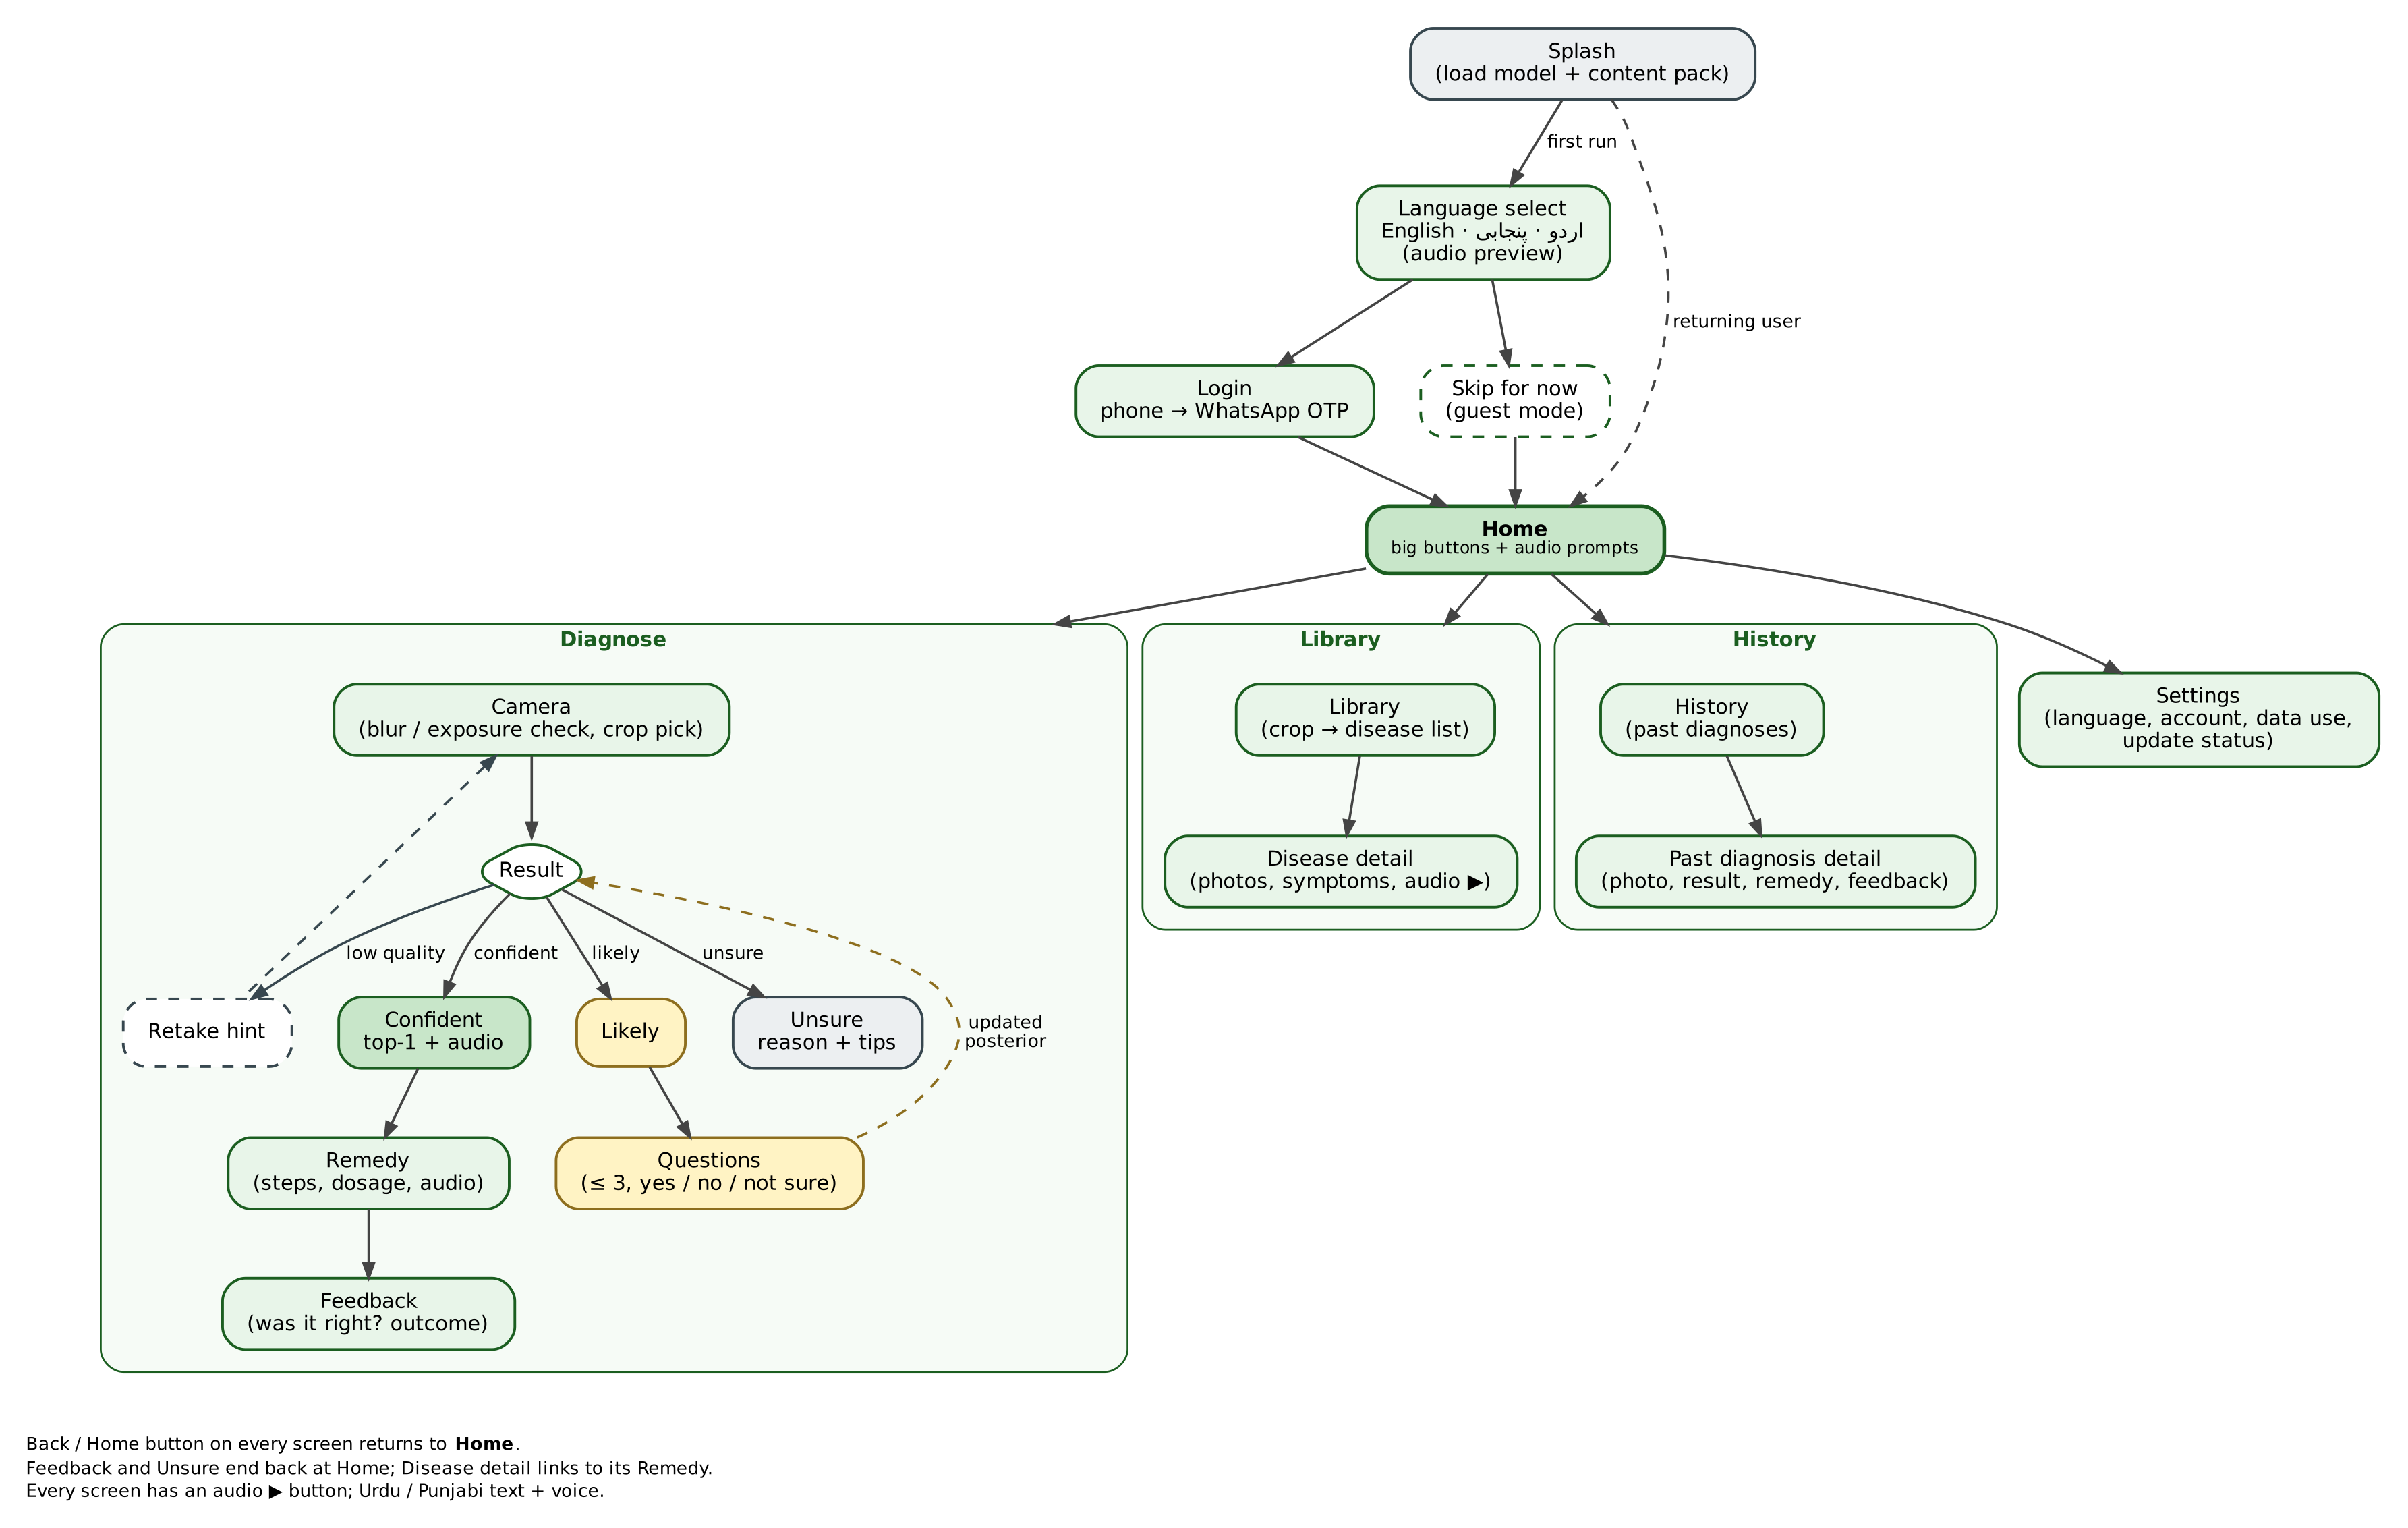
\includegraphics[width=\textwidth,height=0.88\textheight,keepaspectratio]{Figures/diagrams/nav_flow.png}
  \caption{Navigation flow. The primary path Home $\to$ Camera $\to$ Result $\to$ Treatment is four taps; the result branches into Confident, Likely and Unsure states.}
  \label{fig:nav}
\end{figure}

\begin{figure}[H]
  \centering
  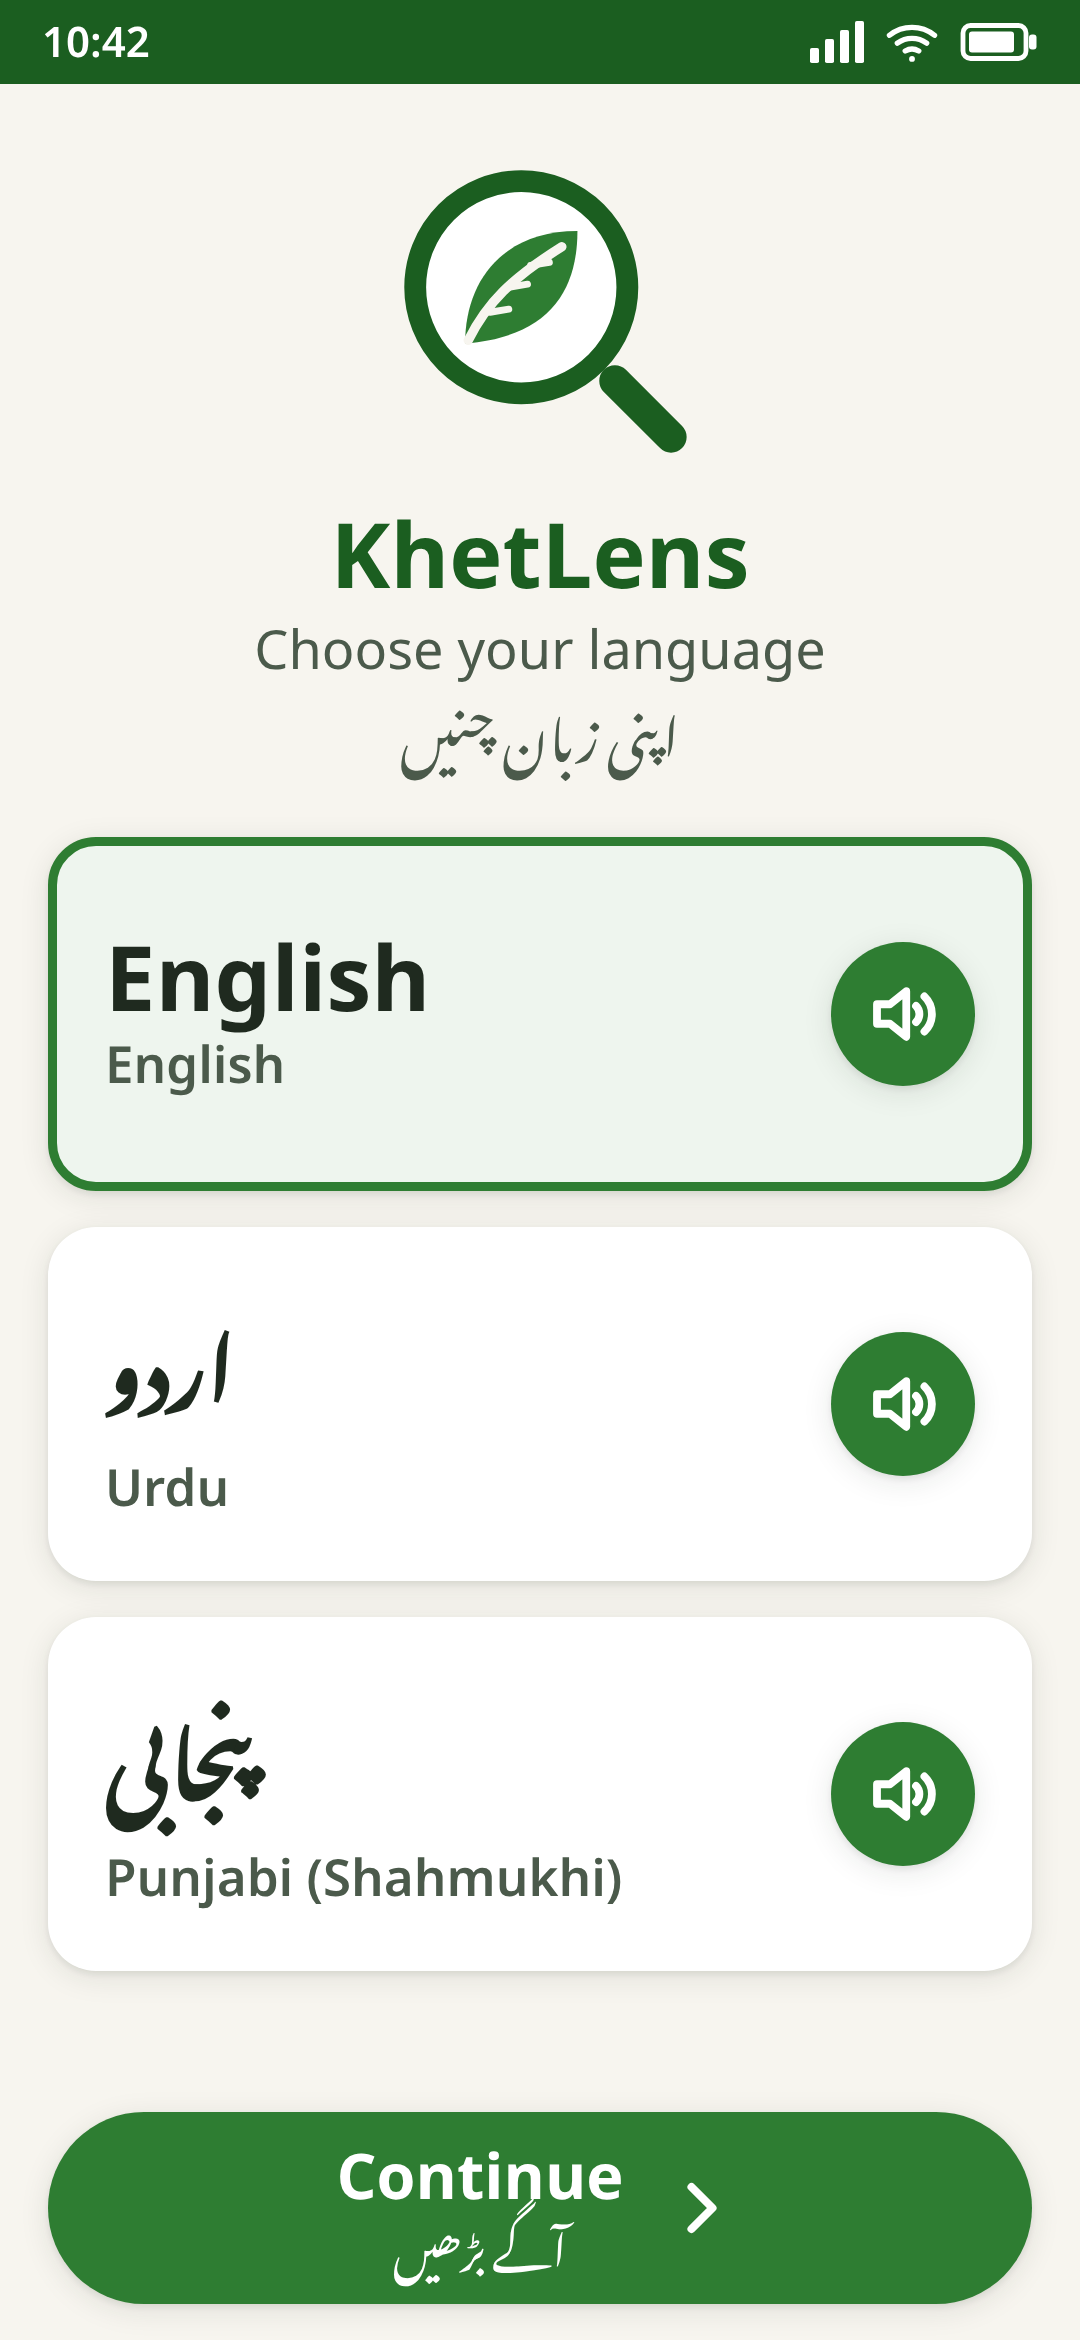
\includegraphics[width=0.3\textwidth]{Figures/gui/01_language.png}\hspace{0.03\textwidth}
  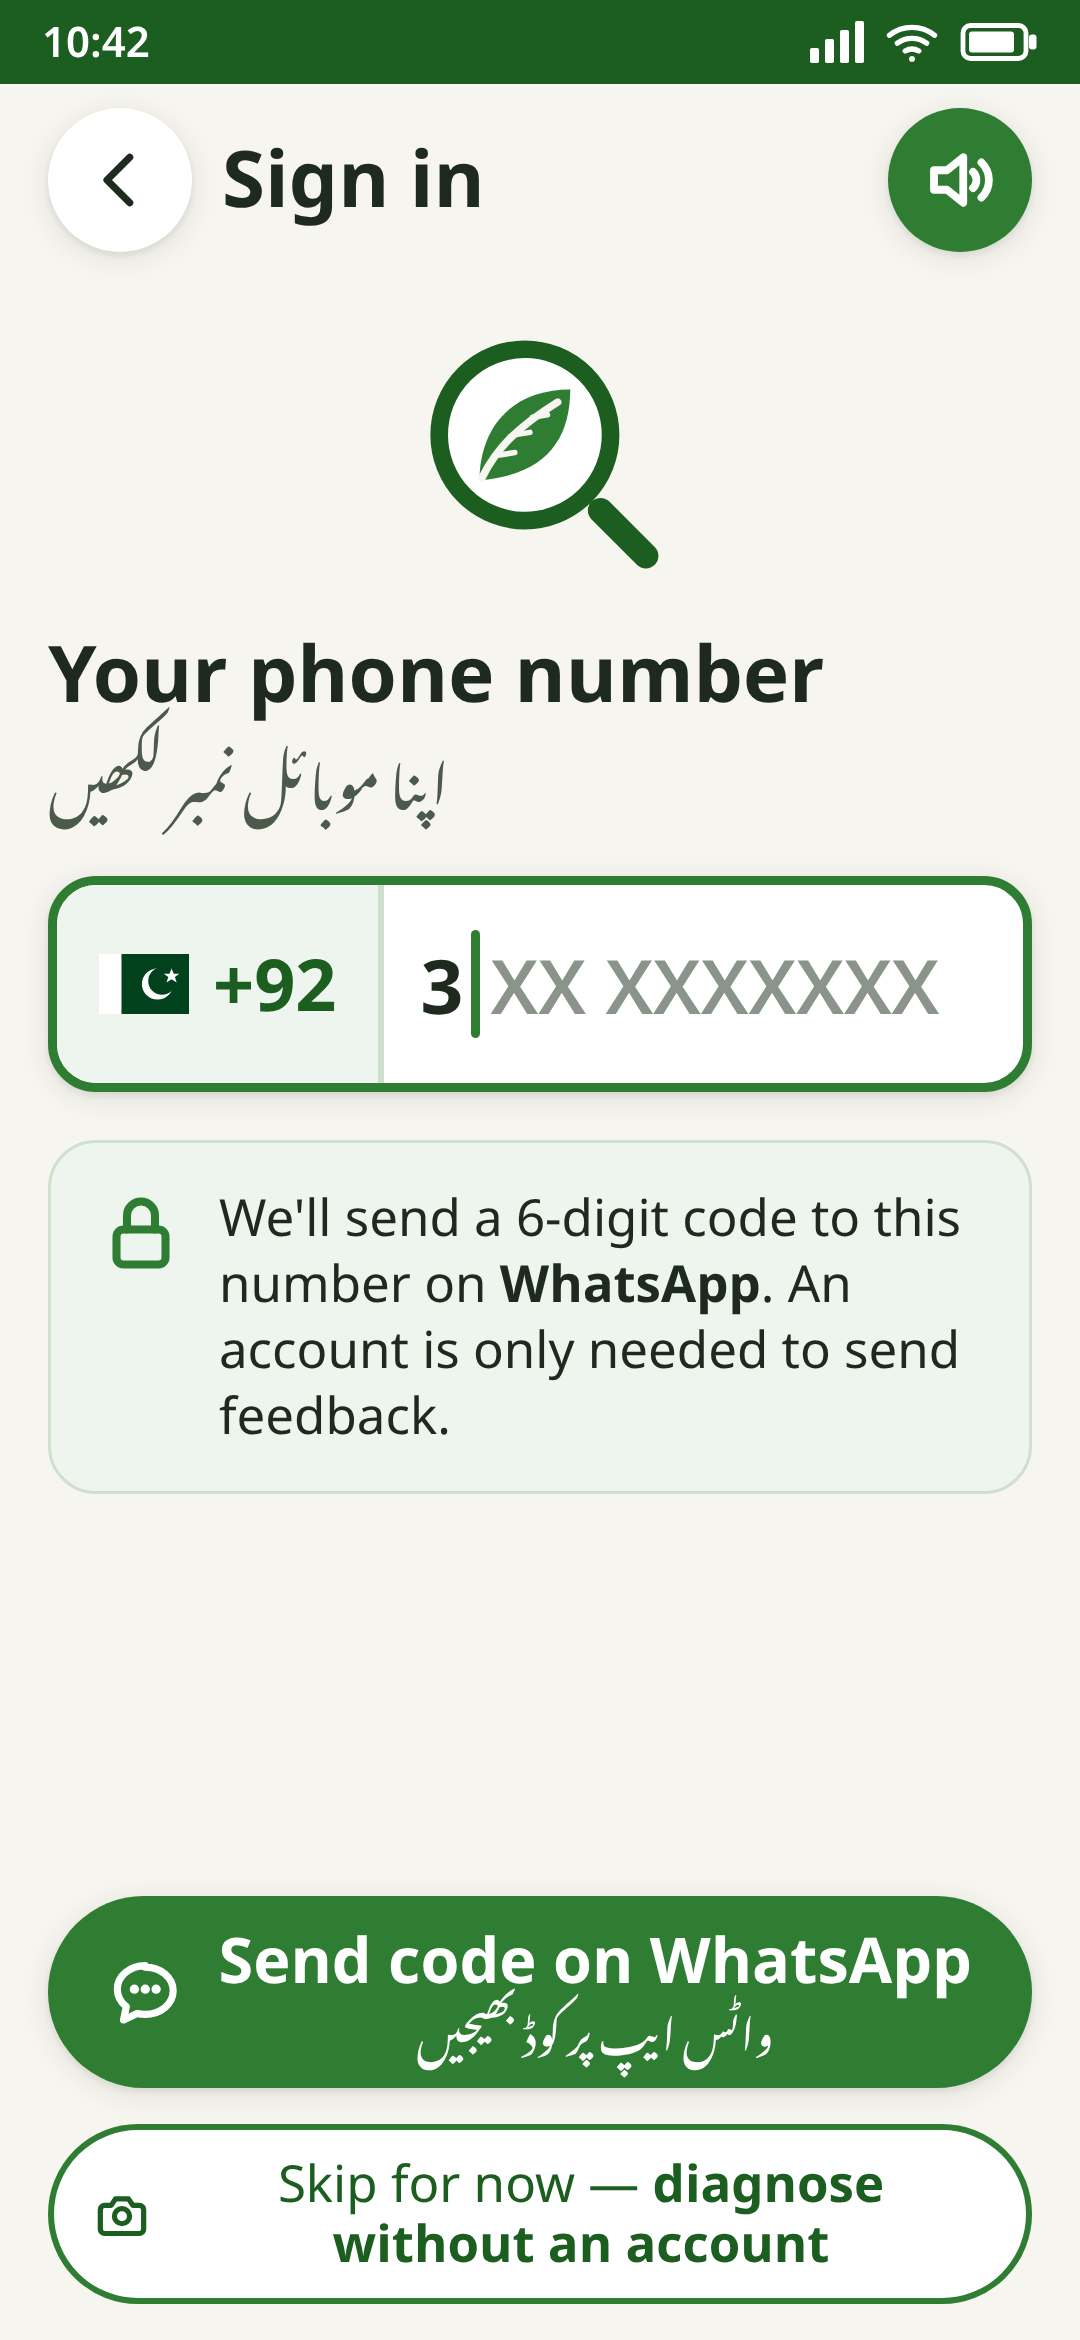
\includegraphics[width=0.3\textwidth]{Figures/gui/02_login.png}\hspace{0.03\textwidth}
  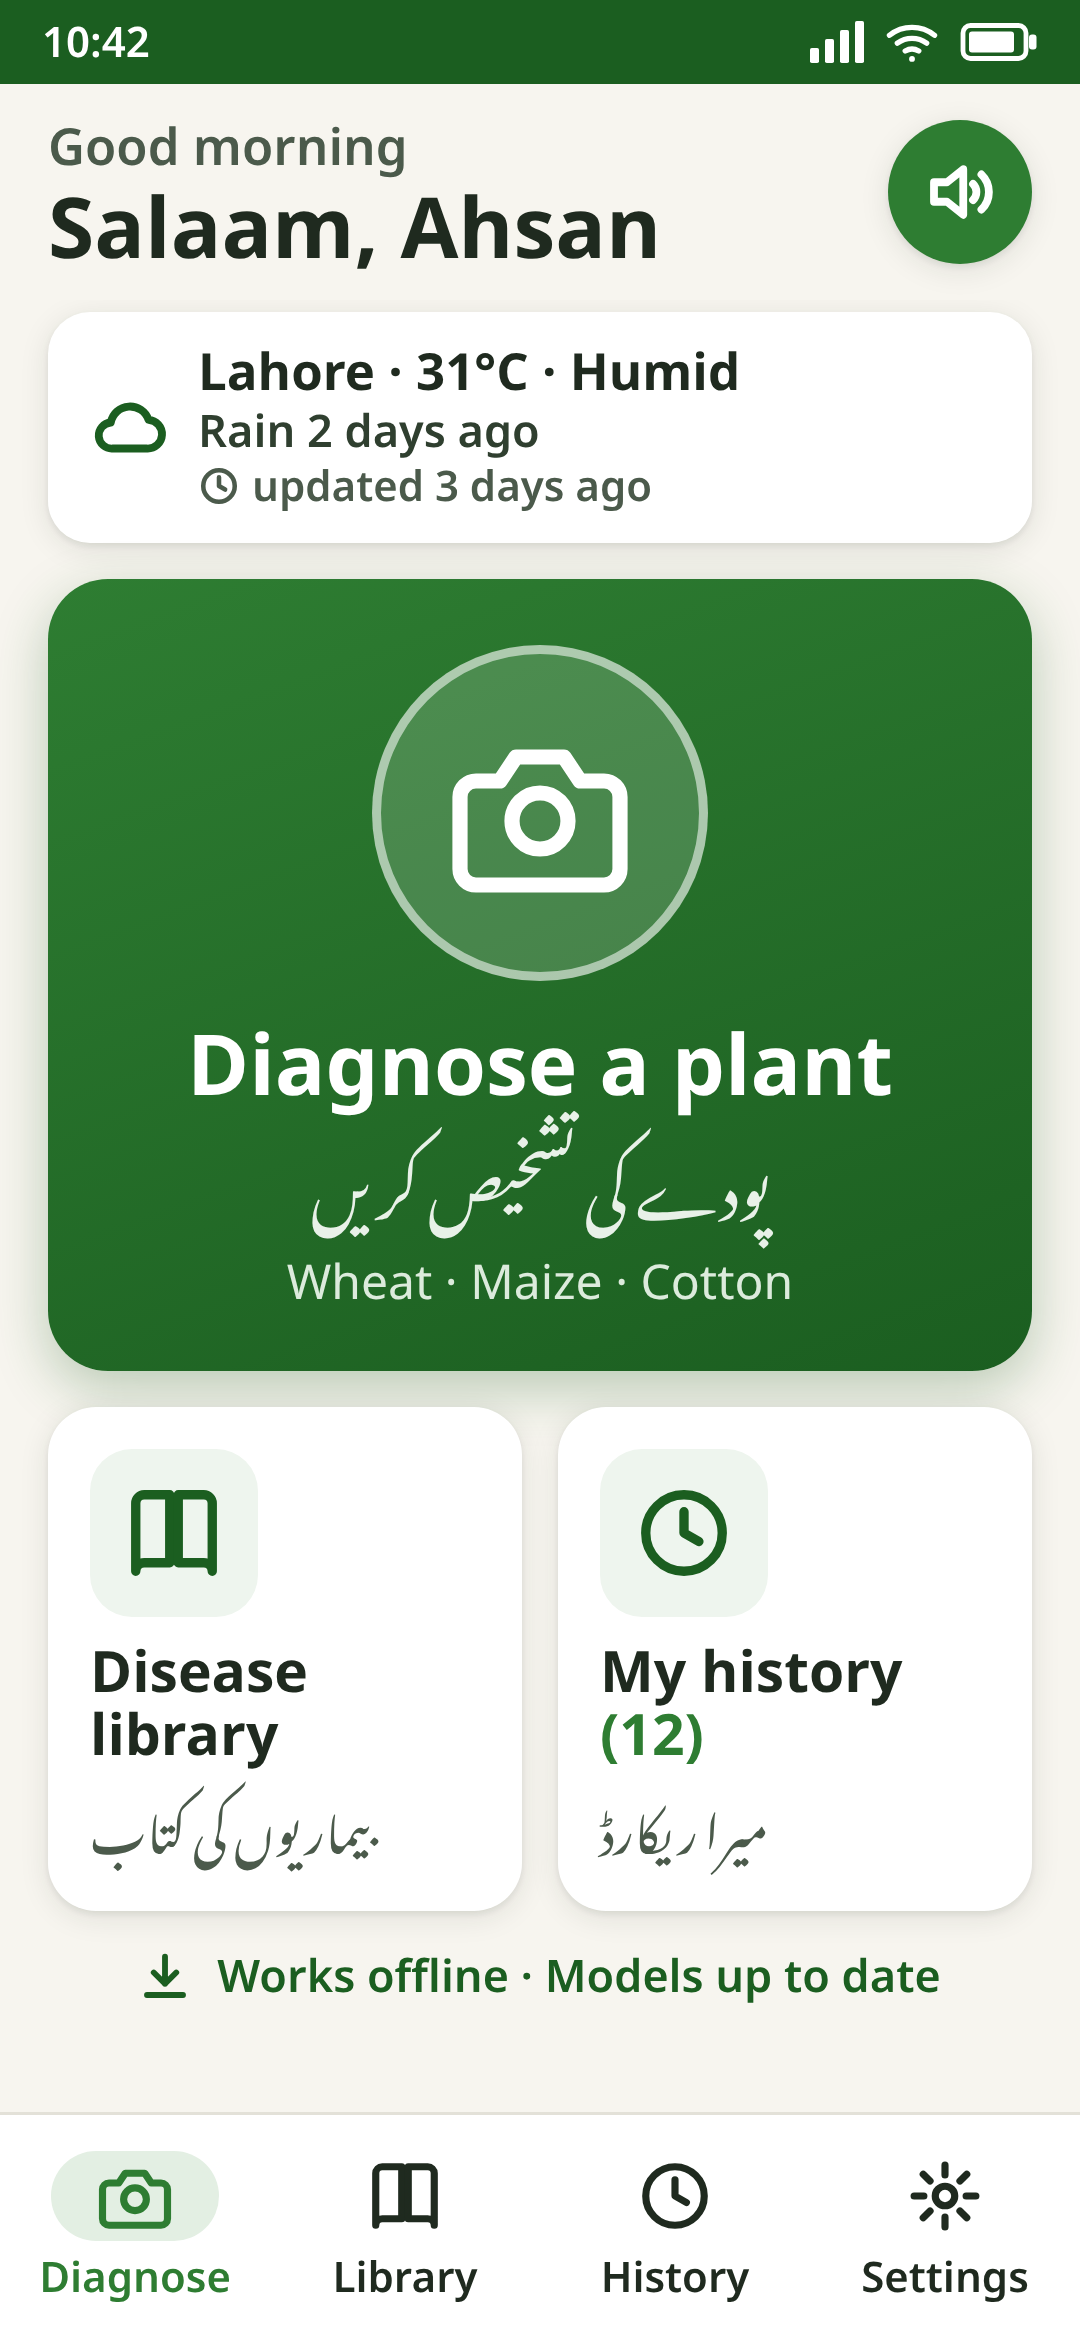
\includegraphics[width=0.3\textwidth]{Figures/gui/03_home.png}
  \caption{Left: language selection with spoken language names (UC-01). Centre: sign-in with a WhatsApp code and the ``Skip for now'' option (UC-02, UC-03). Right: Home with the Diagnose card, the weather chip showing the district and the age of the data (UC-13), and the library and history entries.}
  \label{fig:gui1}
\end{figure}

\begin{figure}[H]
  \centering
  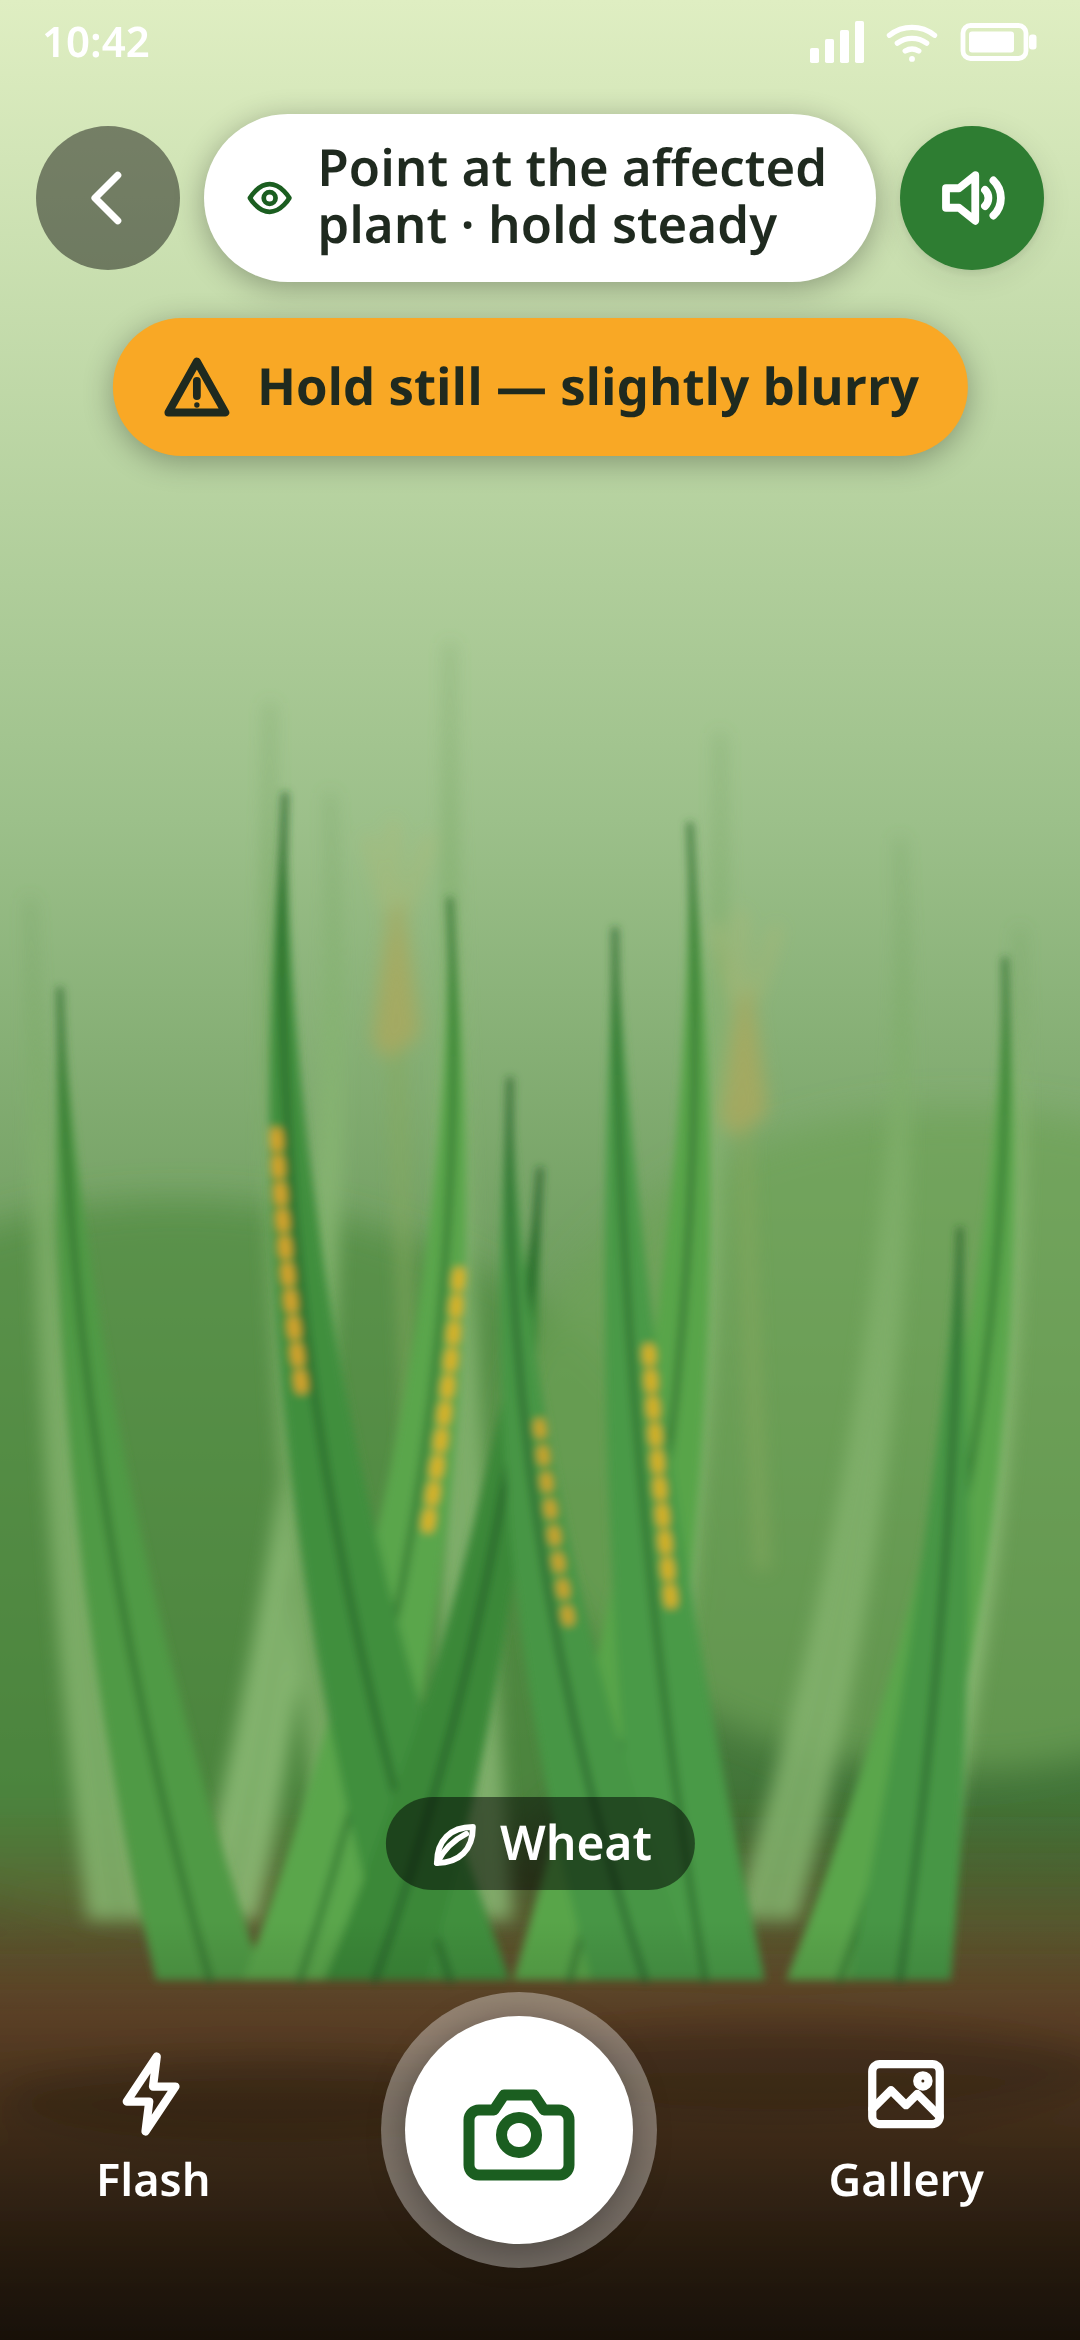
\includegraphics[width=0.3\textwidth]{Figures/gui/04_camera.png}\hspace{0.03\textwidth}
  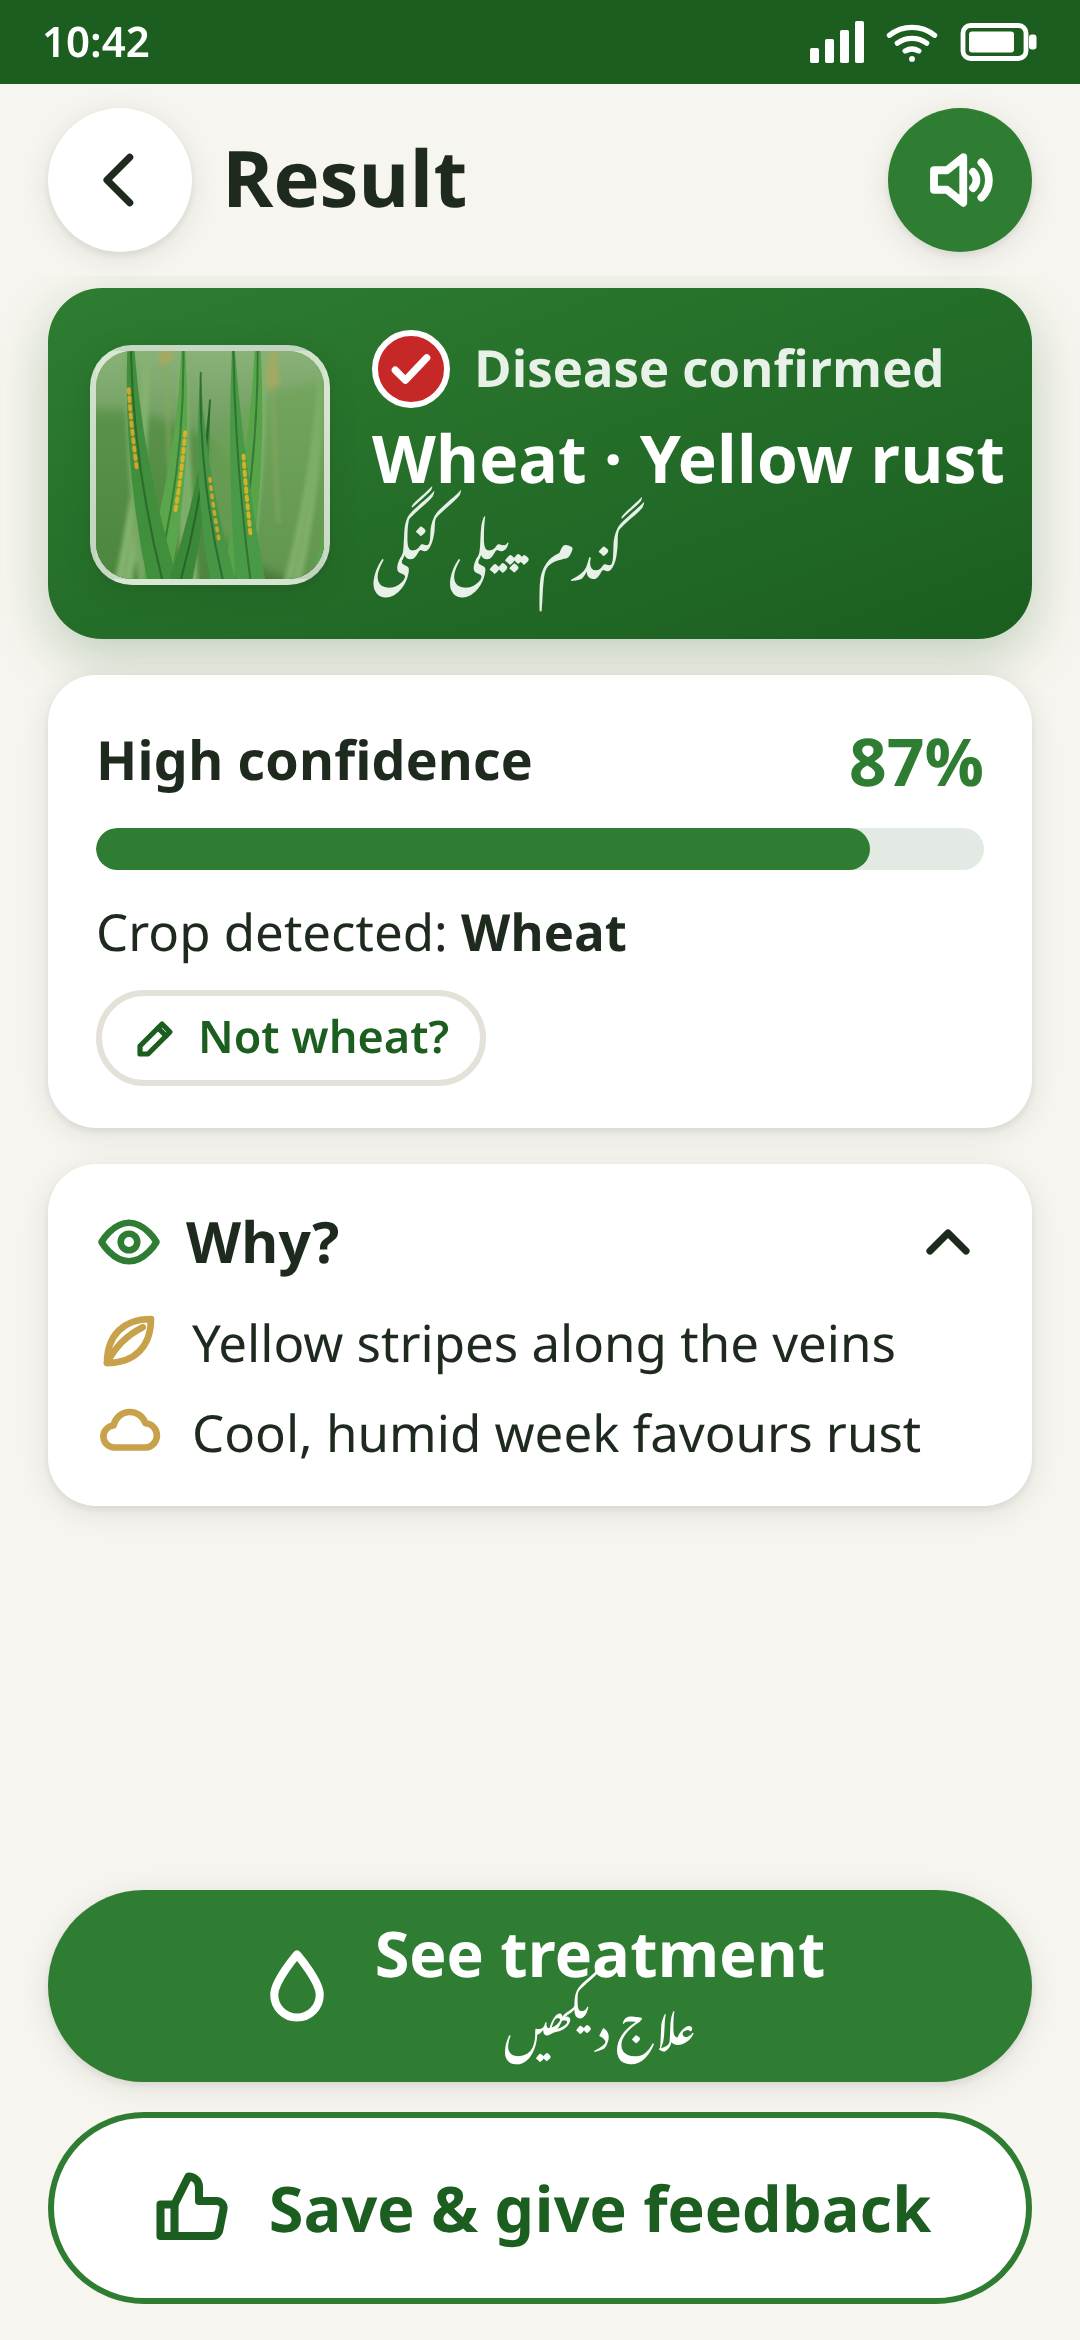
\includegraphics[width=0.3\textwidth]{Figures/gui/05_result_confident.png}\hspace{0.03\textwidth}
  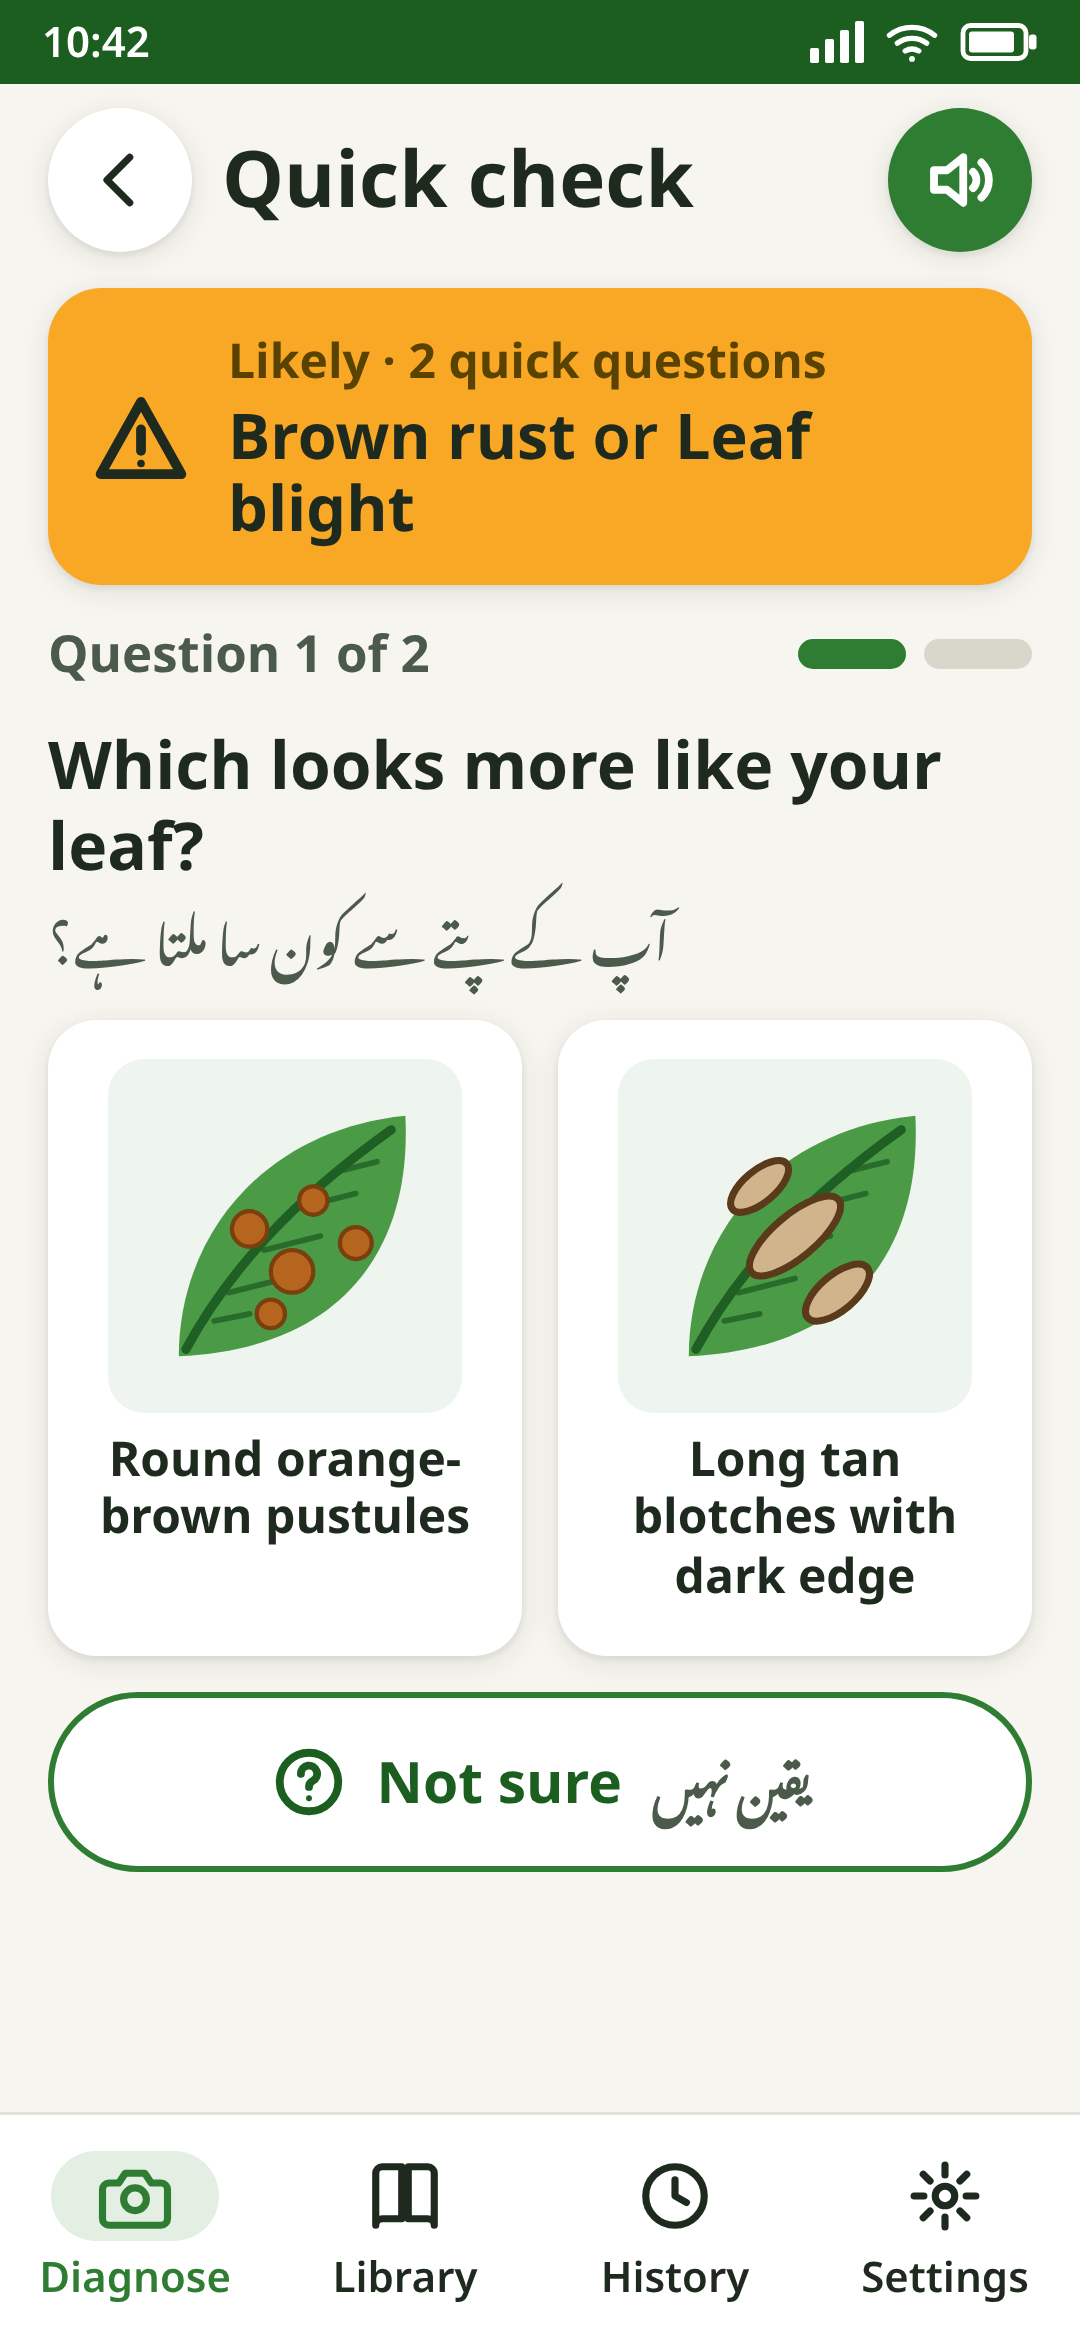
\includegraphics[width=0.3\textwidth]{Figures/gui/06_result_followup.png}
  \caption{Left: camera pointed at the affected plant, with the live blur warning (UC-04). Centre: Confident result with badge, confidence bar, detected-crop chip with correction (UC-05, UC-06) and the Why panel. Right: Likely result asking a picture-based follow-up question (UC-07).}
  \label{fig:gui2}
\end{figure}

\begin{figure}[H]
  \centering
  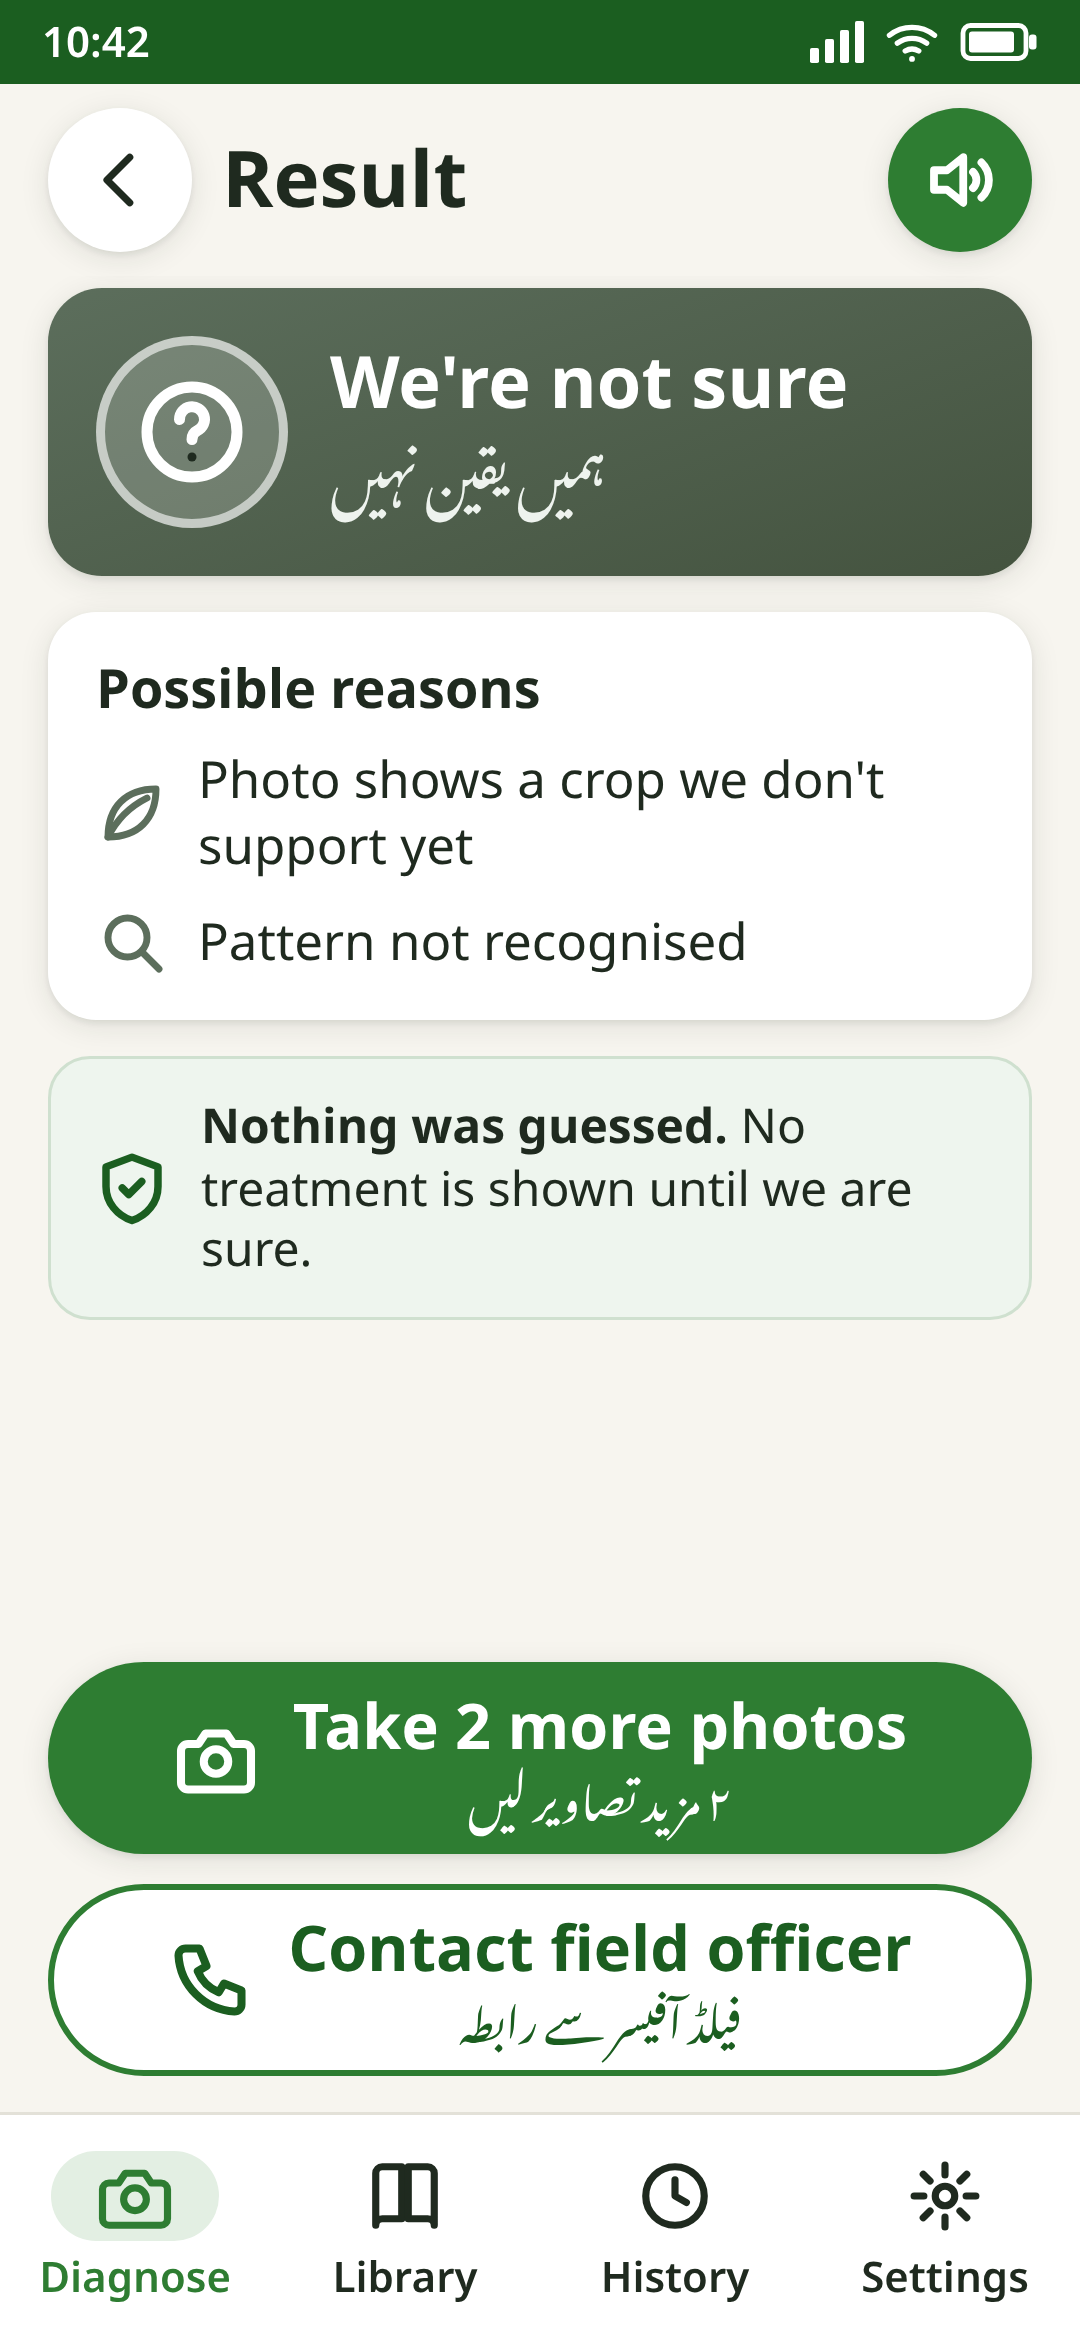
\includegraphics[width=0.3\textwidth]{Figures/gui/07_result_unsure.png}\hspace{0.03\textwidth}
  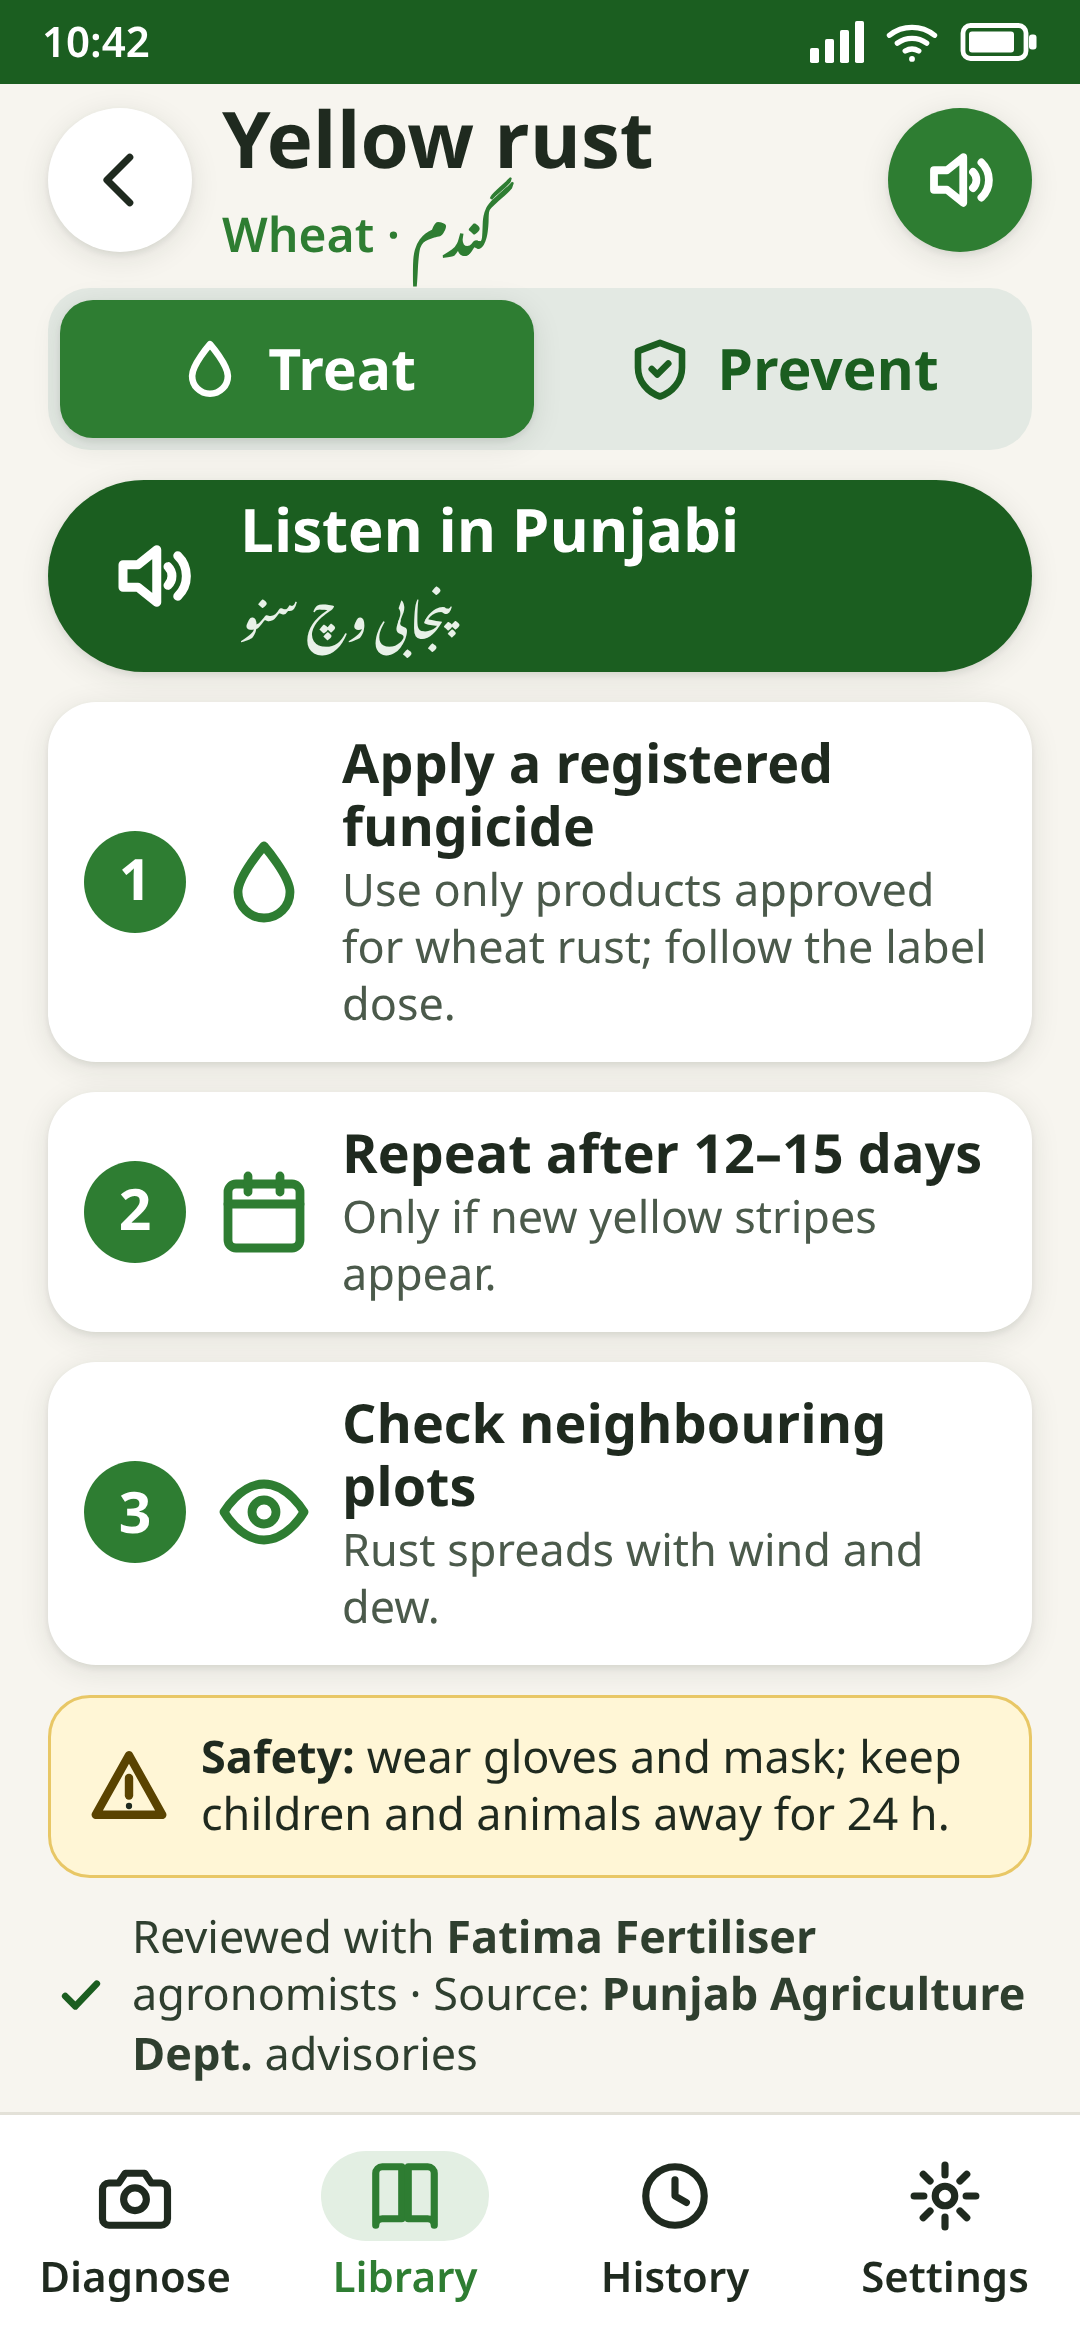
\includegraphics[width=0.3\textwidth]{Figures/gui/08_remedy.png}\hspace{0.03\textwidth}
  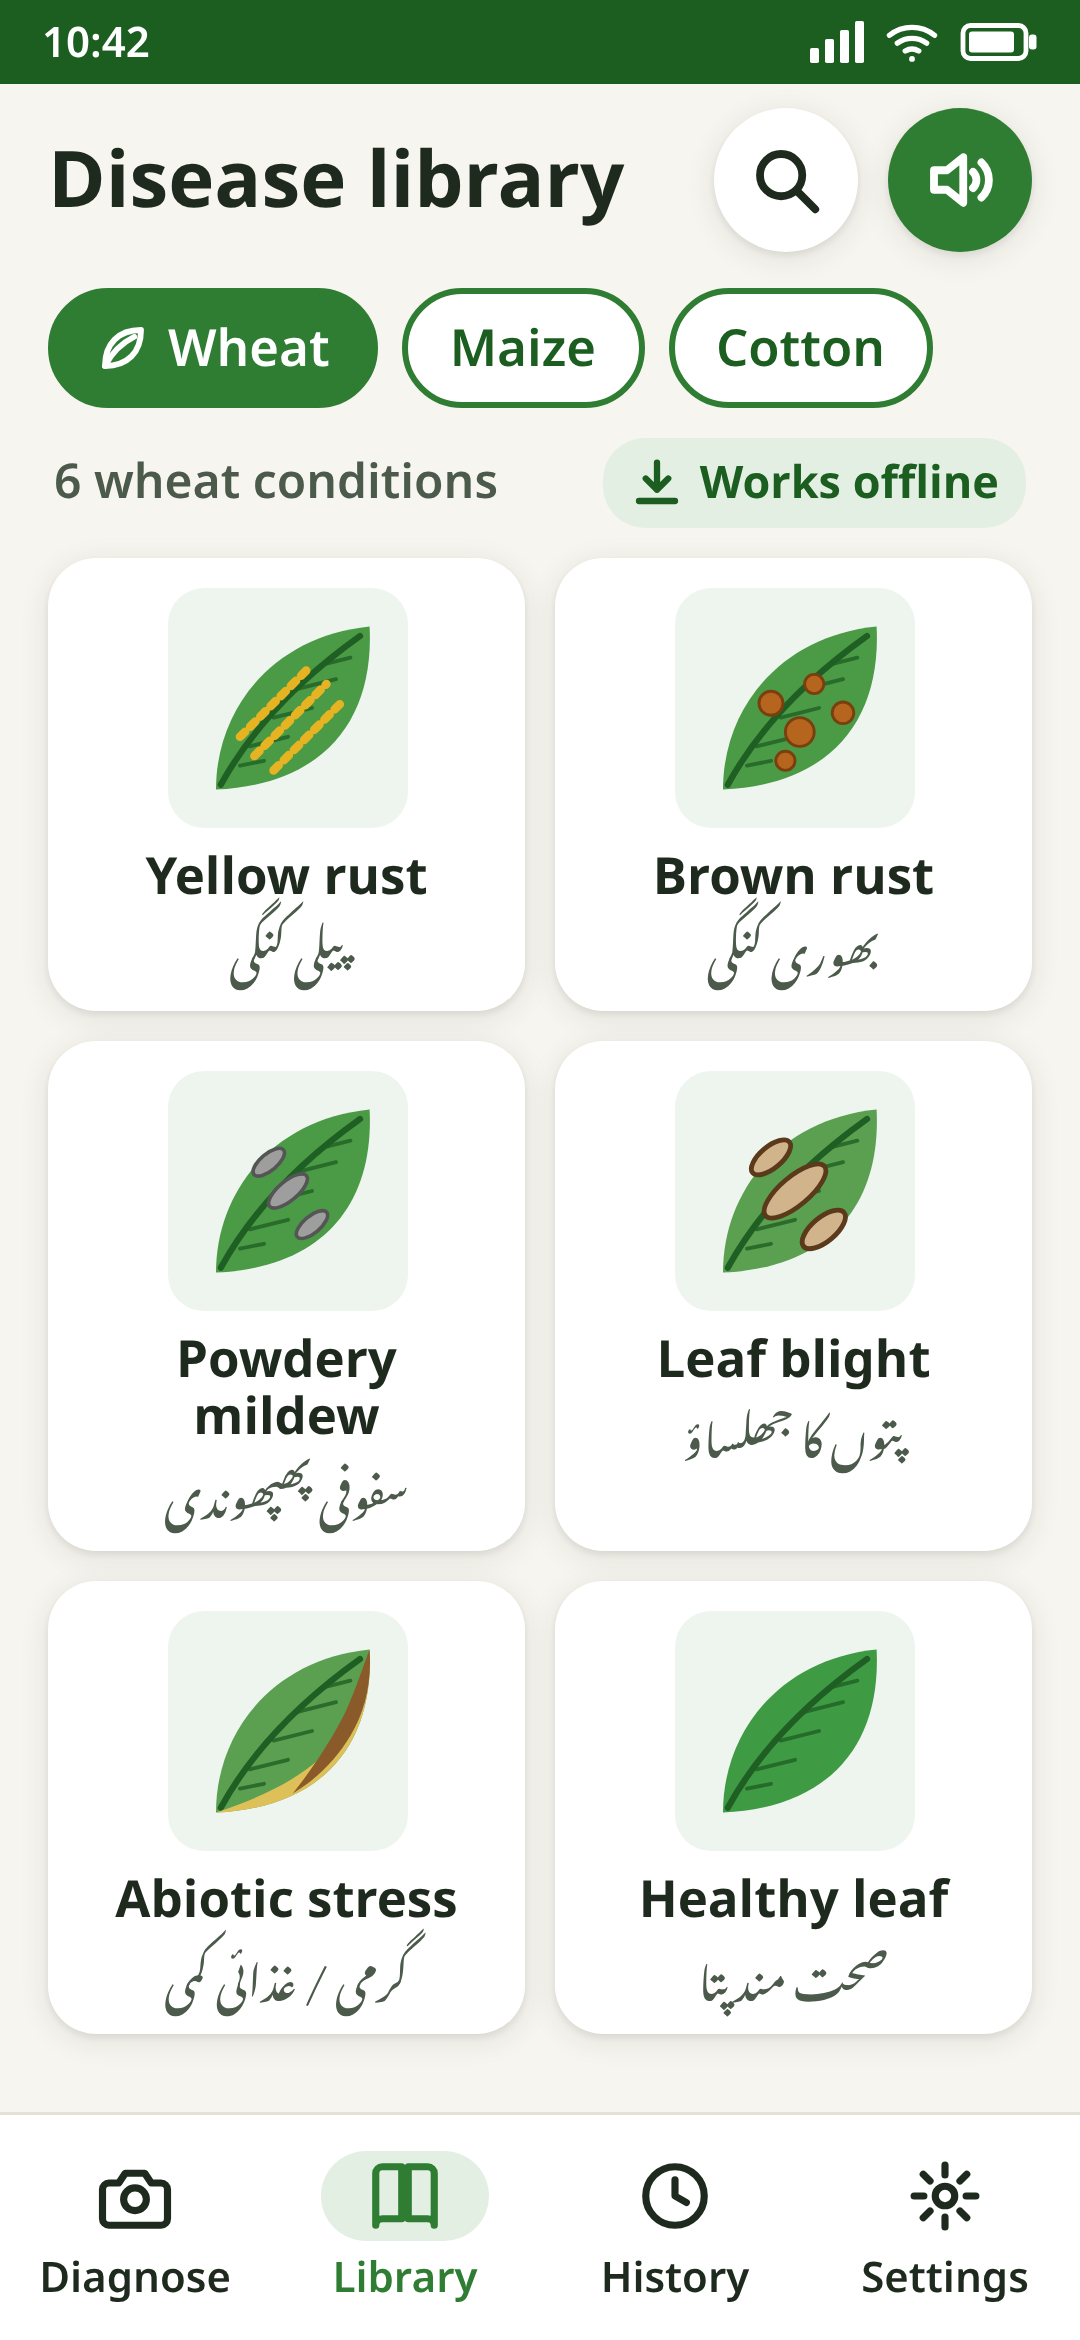
\includegraphics[width=0.3\textwidth]{Figures/gui/09_library.png}
  \caption{Left: Unsure result with reasons and the two actions (UC-08). Centre: treatment screen with Treat and Prevent tabs, numbered steps, safety note, audio button and attribution (UC-09). Right: offline disease library filtered to wheat (UC-10).}
  \label{fig:gui3}
\end{figure}

\begin{figure}[H]
  \centering
  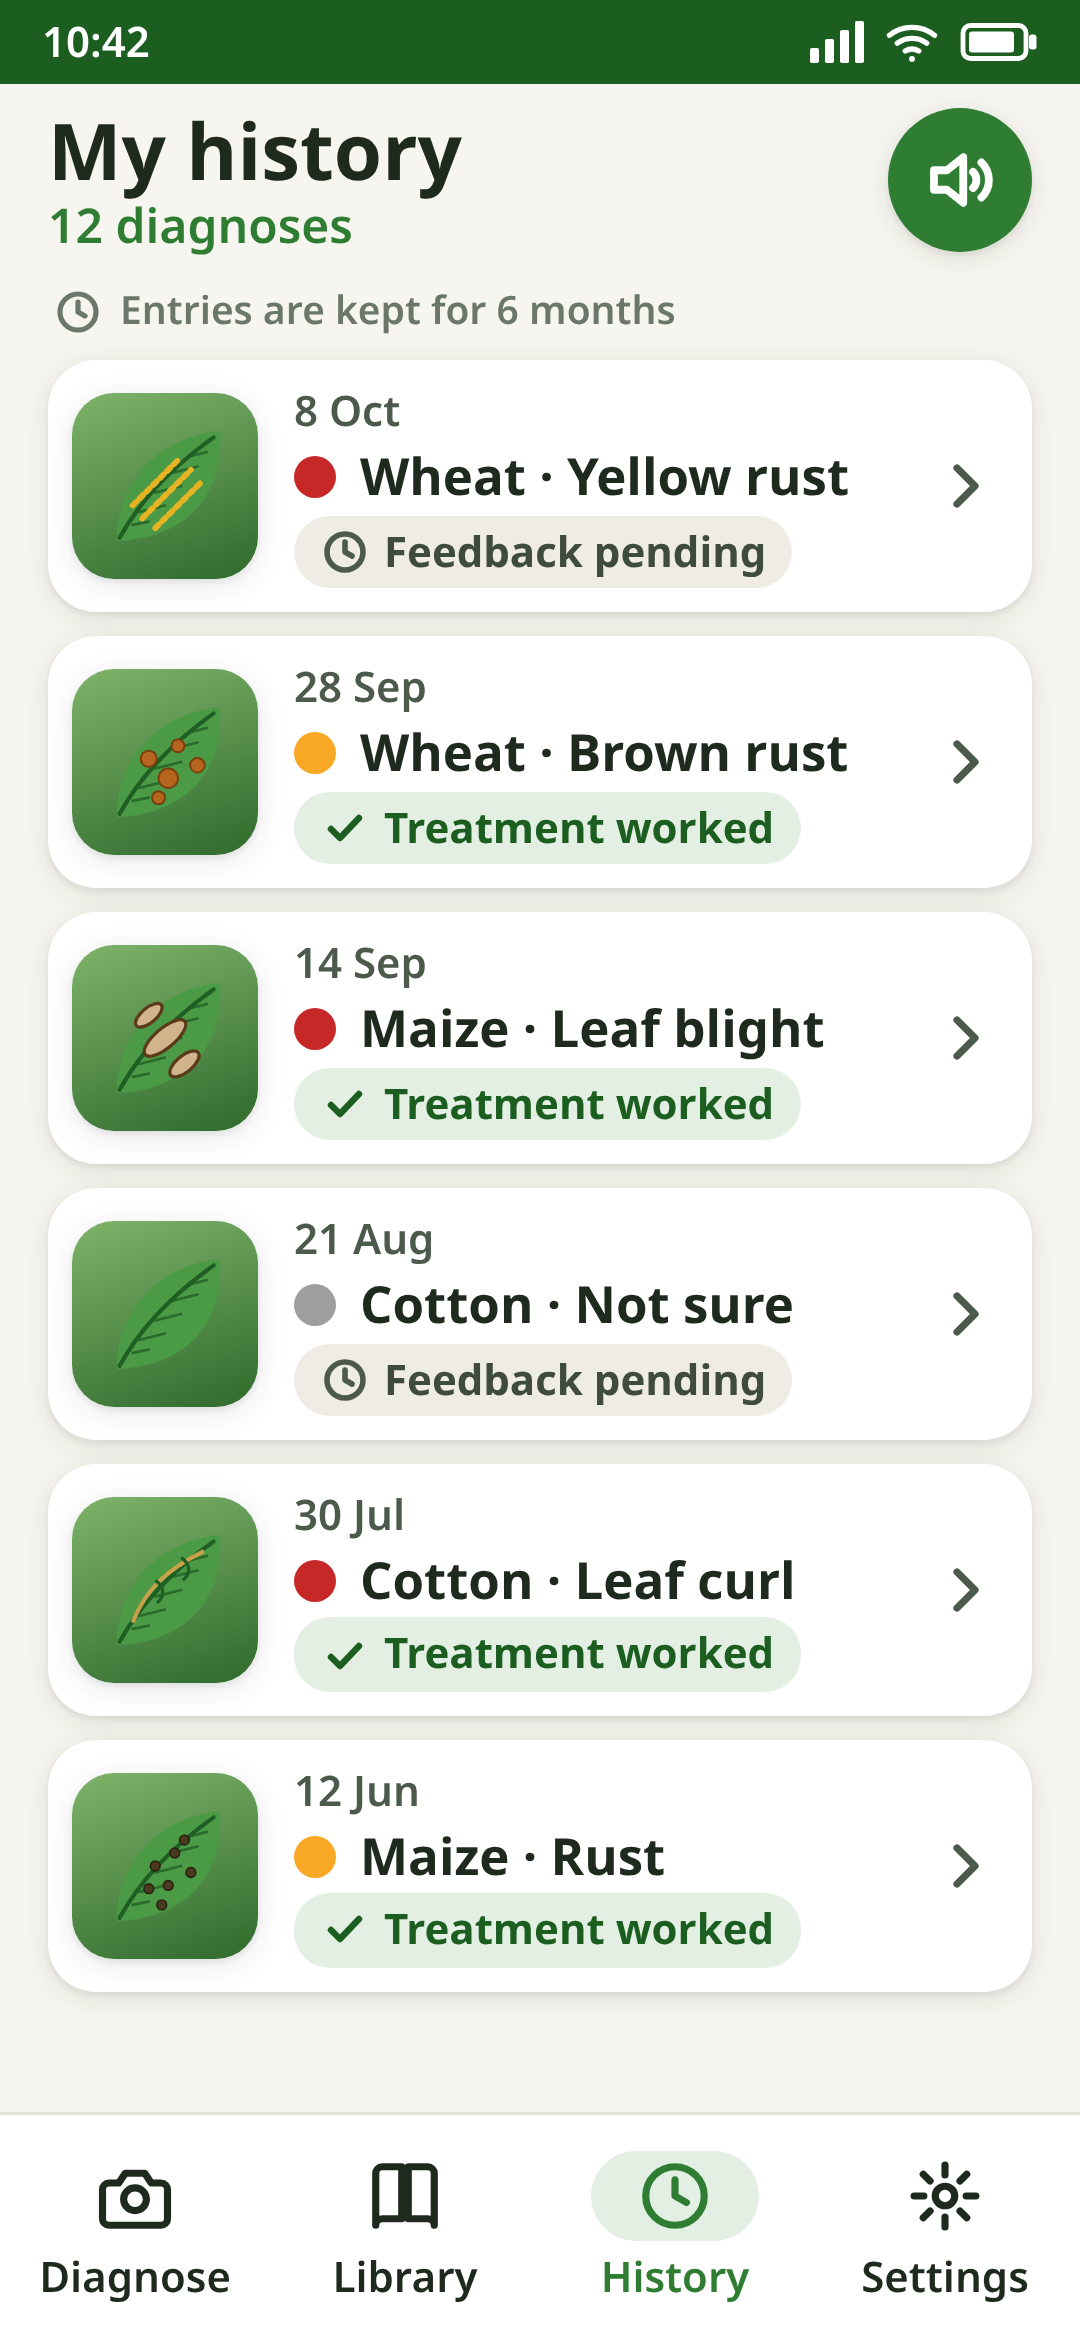
\includegraphics[width=0.3\textwidth]{Figures/gui/10_history.png}\hspace{0.03\textwidth}
  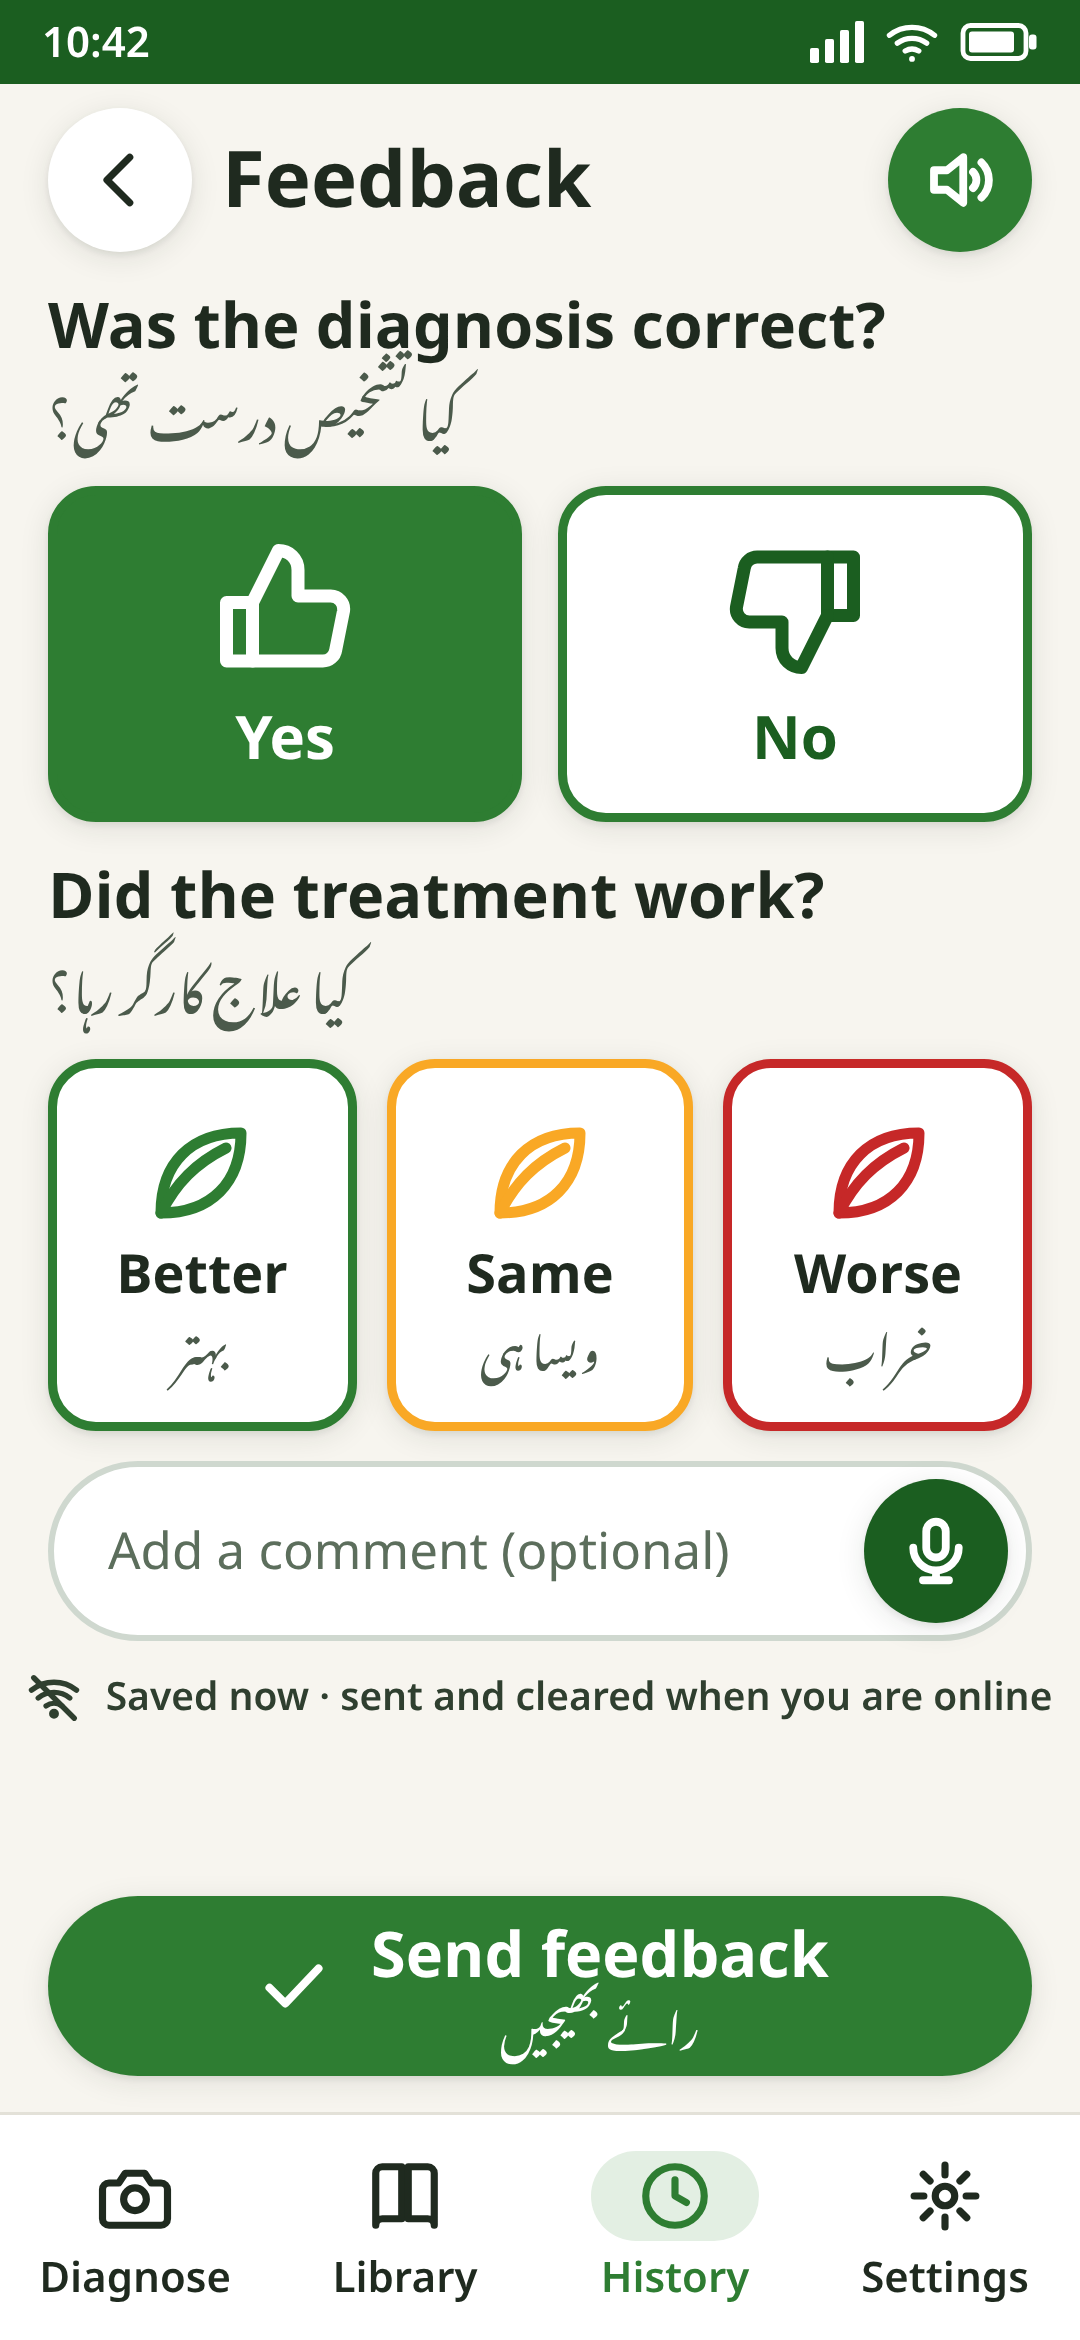
\includegraphics[width=0.3\textwidth]{Figures/gui/11_feedback.png}
  \caption{Left: history of recent diagnoses with outcome colours and feedback status (UC-11). Right: feedback screen with large icon options and the ``saved now, sent when online'' note (UC-12).}
  \label{fig:gui4}
\end{figure}

\section{Database Design}
\label{sec:db}
KhetLens has two data stores. On the phone, a Room (SQLite) database holds the farmer's profile, the last six months of diagnoses, weather snapshots and feedback awaiting upload, together with a read-only copy of the content pack for fast lookup. On the server, PostgreSQL holds users, feedback records, shared images (only when the farmer opts in), content and model versions, and the district list. Both are relational because the data are small, well structured and need transactional integrity.

\subsection{ER Diagram}
Figure~\ref{fig:er} shows the two stores. The phone holds everything the farmer needs; the server holds only what is needed for verification, feedback aggregation and distribution.

\begin{figure}[H]
  \centering
  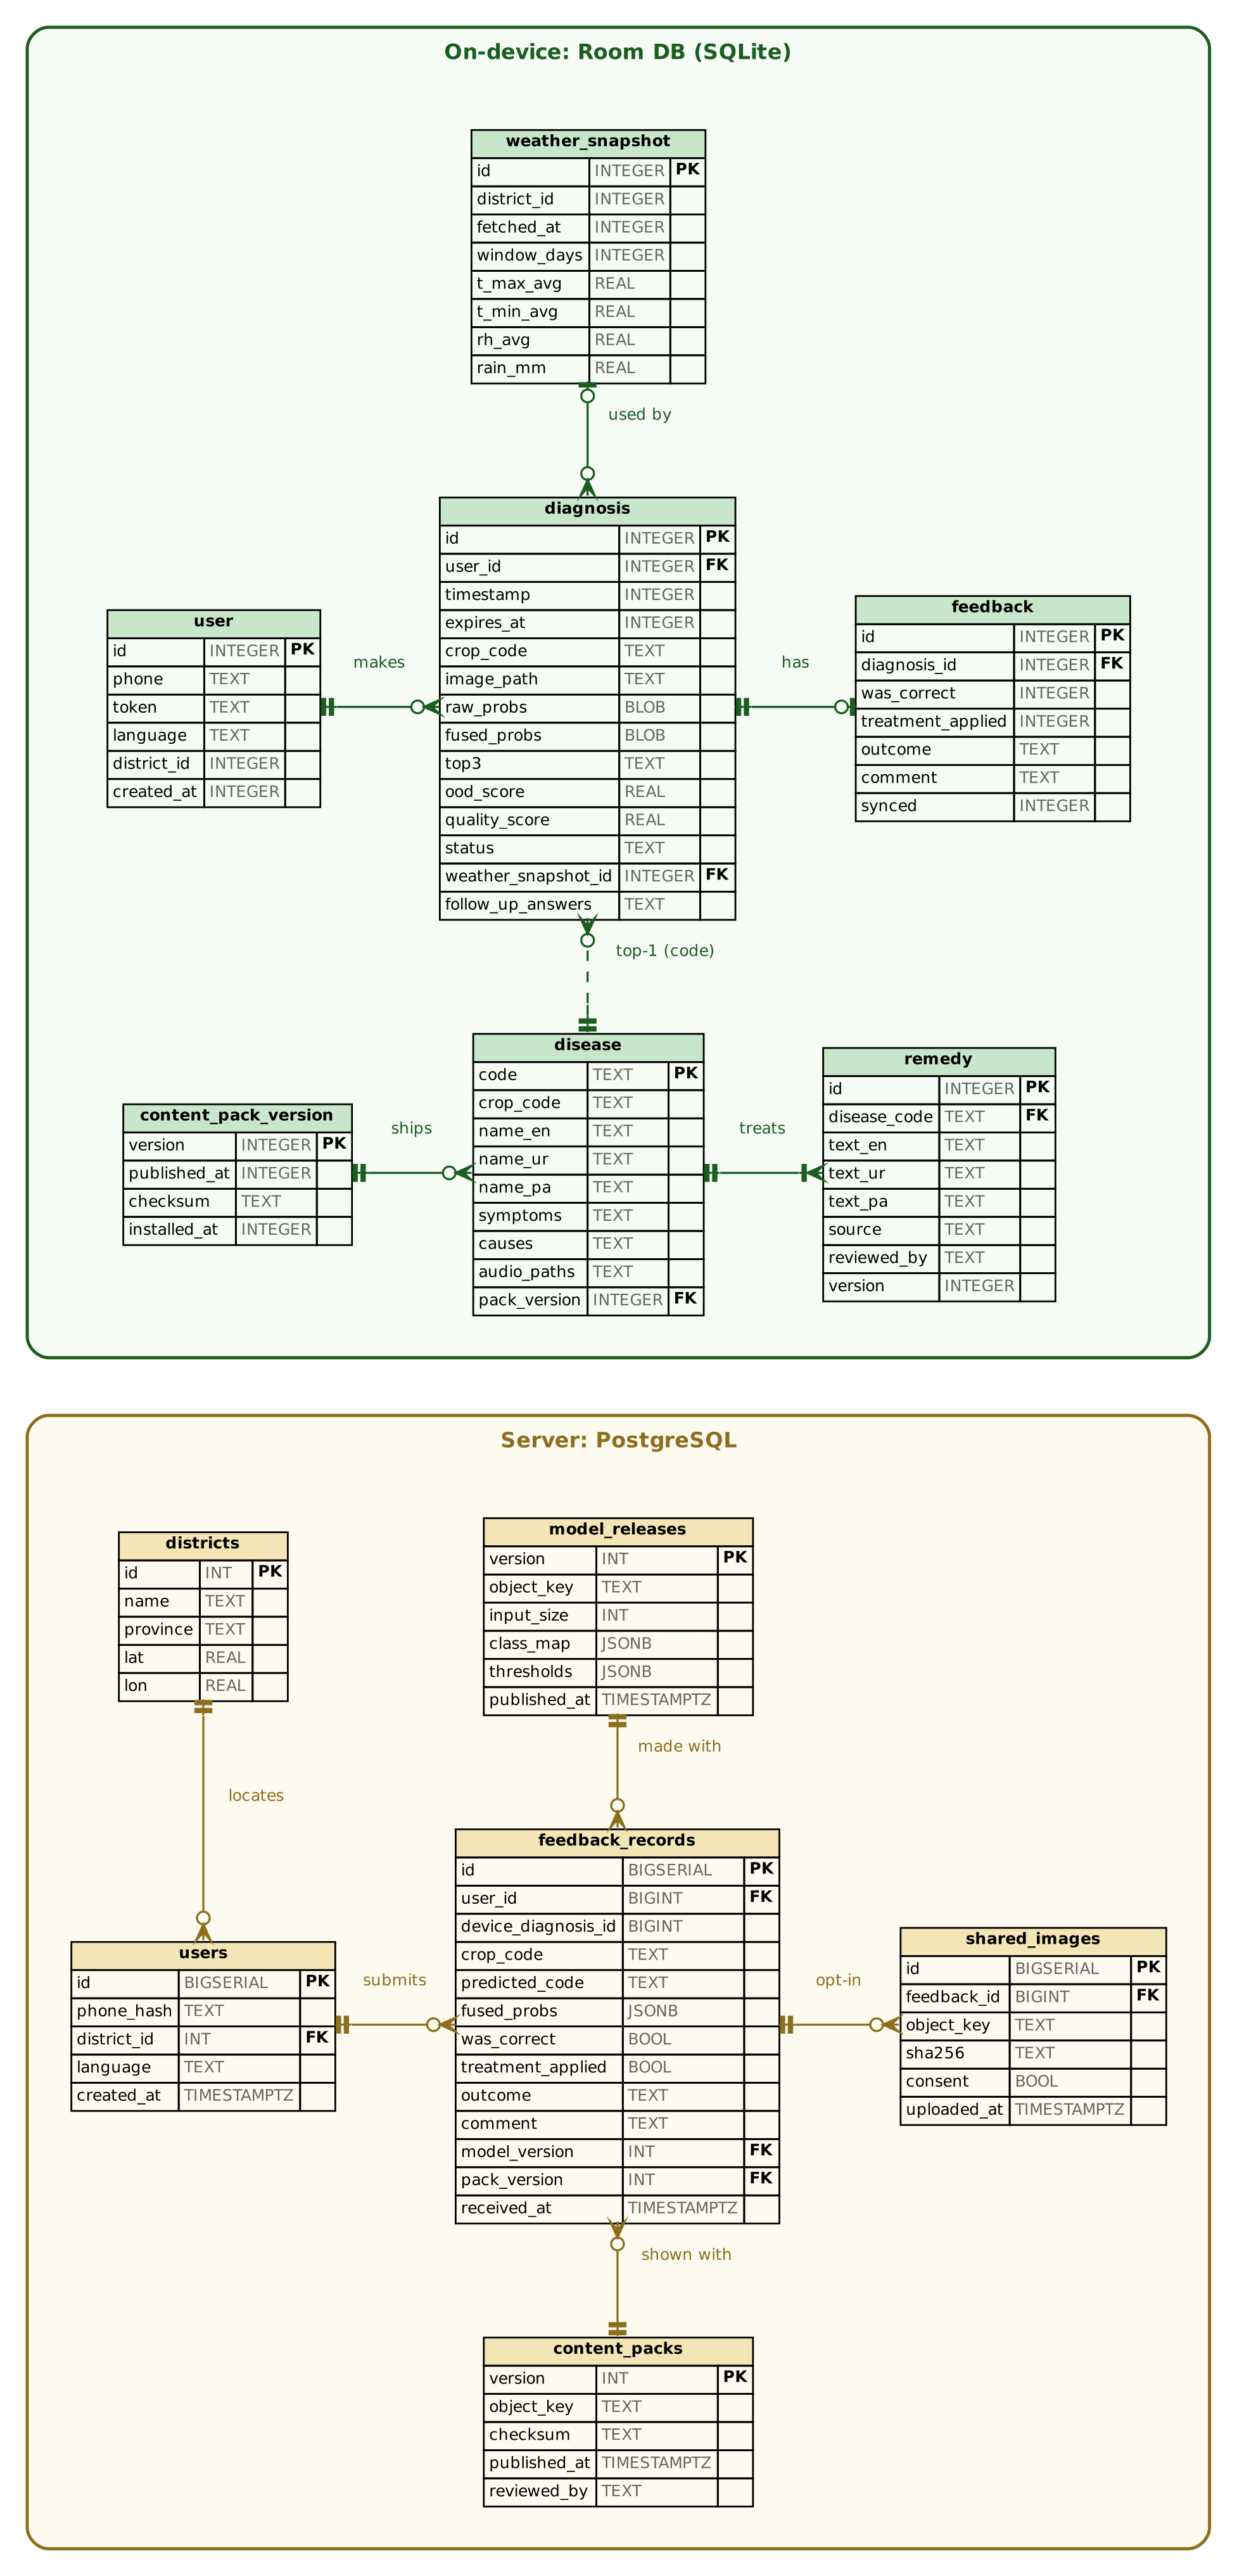
\includegraphics[width=\textwidth,height=0.88\textheight,keepaspectratio]{Figures/diagrams/er_diagram.png}
  \caption{Entity-relationship diagram of the on-device database (top) and the server database (bottom).}
  \label{fig:er}
\end{figure}

\subsection{Data Dictionary}
Tables~\ref{tab:dd-device} and~\ref{tab:dd-server} list every table of the two stores, one attribute per row. PK marks a primary key and FK a foreign key.

\newcommand{\ddtable}[1]{\multicolumn{3}{|l|}{\cellcolor{gray!12}\textbf{Table: #1}} \\ \hline}
{\small
\begin{longtable}{|L{4.0cm}|L{2.6cm}|L{8.0cm}|}
\caption{Data dictionary: on-device database.}\label{tab:dd-device}\\
\hline
\textbf{Attribute} & \textbf{Type} & \textbf{Description} \\ \hline
\endfirsthead
\multicolumn{3}{l}{\small\textit{Table \thetable\ continued}}\\ \hline
\textbf{Attribute} & \textbf{Type} & \textbf{Description} \\ \hline
\endhead
\hline \multicolumn{3}{r}{\small\textit{continued on next page}}\\
\endfoot
\endlastfoot
\ddtable{user}
id (PK) & TEXT & Local profile identifier. \\ \hline
phone & TEXT, null & Mobile number; null for guests. \\ \hline
token & TEXT, null & Reference to the sign-in token in encrypted storage. \\ \hline
language & TEXT & en, ur or pa. \\ \hline
district\_id (FK) & INTEGER & Farmer's district. \\ \hline
created\_at & INTEGER & Profile creation time. \\ \hline
\ddtable{diagnosis}
id (PK) & TEXT & Diagnosis identifier. \\ \hline
user\_id (FK) & TEXT & Owner. \\ \hline
timestamp & INTEGER & Capture time. \\ \hline
expires\_at & INTEGER & Automatic deletion time (six months after capture). \\ \hline
crop\_code & TEXT & WHT, MZE or COT. \\ \hline
crop\_corrected & INTEGER & 1 if the farmer changed the detected crop. \\ \hline
image\_path & TEXT & App-private path of the photograph. \\ \hline
raw\_probs & JSON & Class probabilities before the weather prior. \\ \hline
fused\_probs & JSON & Class probabilities after the weather prior. \\ \hline
top1\_code (FK) & TEXT, null & Final condition; null for Unsure. \\ \hline
confidence & REAL & Calibrated confidence of the final condition. \\ \hline
ood\_score & REAL & Novelty score (feature distance). \\ \hline
quality\_score & REAL & Image quality score. \\ \hline
status & TEXT & CONFIDENT, LIKELY or UNSURE. \\ \hline
weather\_snapshot\_id (FK) & TEXT, null & Snapshot used, if any. \\ \hline
followup\_answers & JSON & Question and option identifiers. \\ \hline
model\_version & TEXT & Model release used. \\ \hline
\ddtable{weather\_snapshot}
id (PK) & TEXT & Snapshot identifier. \\ \hline
district\_id & INTEGER & District. \\ \hline
fetched\_at & INTEGER & Fetch time. \\ \hline
tmax\_avg & REAL & Mean daily maximum temperature over 14 days. \\ \hline
tmin\_avg & REAL & Mean daily minimum temperature over 14 days. \\ \hline
rh\_avg & REAL & Mean relative humidity over 14 days. \\ \hline
rain\_mm & REAL & Total rainfall over 14 days. \\ \hline
days\_since\_rain & INTEGER & Days since the last rain. \\ \hline
\ddtable{feedback (row deleted once the server acknowledges it)}
id (PK) & TEXT & Feedback identifier. \\ \hline
diagnosis\_id (FK) & TEXT & One feedback per diagnosis. \\ \hline
was\_correct & INTEGER, null & 1 yes, 0 no. \\ \hline
stated\_condition & TEXT, null & Farmer's own answer if ``no''. \\ \hline
outcome & TEXT, null & BETTER, SAME or WORSE. \\ \hline
comment & TEXT, null & Optional comment. \\ \hline
share\_image & INTEGER & 1 if the farmer opted in to share the photograph. \\ \hline
synced & INTEGER & 0 while awaiting upload. \\ \hline
\ddtable{condition}
code (PK) & TEXT & e.g.\ WHT\_YRUST. \\ \hline
crop\_code & TEXT & Crop. \\ \hline
name\_en, name\_ur, name\_pa & TEXT & Names in the three languages. \\ \hline
symptoms, causes & JSON & Per-language text. \\ \hline
audio\_paths & JSON & Per-language audio files. \\ \hline
\ddtable{remedy}
id (PK) & TEXT & Guidance identifier. \\ \hline
condition\_code (FK) & TEXT & Condition. \\ \hline
kind & TEXT & TREAT or PREVENT. \\ \hline
steps & JSON & Ordered per-language steps. \\ \hline
safety\_note & JSON & Per-language safety note. \\ \hline
source, reviewed\_by, reviewed\_on & TEXT & Attribution (mandatory). \\ \hline
\ddtable{content\_pack\_version}
version (PK) & TEXT & Installed content version. \\ \hline
checksum & TEXT & Checksum of the installed pack. \\ \hline
installed\_at & INTEGER & Install time. \\ \hline
\end{longtable}
}

{\small
\begin{longtable}{|L{4.0cm}|L{2.6cm}|L{8.0cm}|}
\caption{Data dictionary: server database.}\label{tab:dd-server}\\
\hline
\textbf{Attribute} & \textbf{Type} & \textbf{Description} \\ \hline
\endfirsthead
\multicolumn{3}{l}{\small\textit{Table \thetable\ continued}}\\ \hline
\textbf{Attribute} & \textbf{Type} & \textbf{Description} \\ \hline
\endhead
\hline \multicolumn{3}{r}{\small\textit{continued on next page}}\\
\endfoot
\endlastfoot
\ddtable{users}
id (PK) & UUID & Server user identifier. \\ \hline
phone\_hash & TEXT & Salted hash of the number; the number itself is not kept. \\ \hline
district\_id (FK) & INTEGER & District. \\ \hline
language & TEXT & Preferred language. \\ \hline
created\_at, last\_seen & TIMESTAMP & Audit fields. \\ \hline
\ddtable{feedback\_records}
id (PK) & UUID & Mirrors the device feedback id. \\ \hline
user\_id (FK) & UUID & Submitter. \\ \hline
district\_id (FK) & INTEGER & District at diagnosis. \\ \hline
crop\_code, predicted\_code & TEXT & Crop and condition predicted by the model. \\ \hline
status, confidence & TEXT, REAL & Outcome and calibrated confidence. \\ \hline
was\_correct & SMALLINT & Farmer's answer. \\ \hline
stated\_condition & TEXT & Farmer's own answer if ``no''. \\ \hline
outcome, comment & TEXT & Treatment outcome and comment. \\ \hline
model\_version, pack\_version (FK) & TEXT & Versions in use. \\ \hline
diagnosed\_at, received\_at & TIMESTAMP & Timestamps. \\ \hline
\ddtable{shared\_images (only when the farmer opted in)}
id (PK) & UUID & Image identifier. \\ \hline
feedback\_id (FK) & UUID & Linked feedback. \\ \hline
object\_key & TEXT & Storage key. \\ \hline
label\_status & TEXT & UNLABELLED, LABELLED or REJECTED. \\ \hline
\ddtable{content\_packs}
version (PK) & TEXT & Semantic version. \\ \hline
object\_key, checksum & TEXT & File location and checksum. \\ \hline
published\_at & TIMESTAMP & Release time. \\ \hline
reviewed\_by & TEXT & Reviewing agronomist. \\ \hline
\ddtable{model\_releases}
version (PK) & TEXT & Semantic version. \\ \hline
object\_key, checksum & TEXT & File location and checksum. \\ \hline
input\_size & INTEGER & Model input size in pixels. \\ \hline
class\_map & JSON & Class indices to condition codes. \\ \hline
thresholds & JSON & Thresholds used by the uncertainty check. \\ \hline
field\_macro\_f1 & REAL & Acceptance metric for the release. \\ \hline
published\_at & TIMESTAMP & Release time. \\ \hline
\ddtable{districts}
id (PK) & INTEGER & District identifier. \\ \hline
name\_en, name\_ur & TEXT & Names. \\ \hline
centroid\_lat, centroid\_lon & REAL & Centroid for weather queries. \\ \hline
\end{longtable}
}

\section{Risk Analysis}
\label{sec:risks}
{\small
\begin{longtable}{|L{0.9cm}|L{4.2cm}|L{0.5cm}|L{0.5cm}|L{7.7cm}|}
\caption{Risk register. L = likelihood, I = impact, each rated High (H), Medium (M) or Low (L).}\label{tab:risks}\\
\hline
\textbf{ID} & \textbf{Risk} & \textbf{L} & \textbf{I} & \textbf{Mitigation} \\ \hline
\endfirsthead
\multicolumn{5}{l}{\small\textit{Table \thetable\ continued}}\\ \hline
\textbf{ID} & \textbf{Risk} & \textbf{L} & \textbf{I} & \textbf{Mitigation} \\ \hline
\endhead
\hline \multicolumn{5}{r}{\small\textit{continued on next page}}\\
\endfoot
\endlastfoot
R-01 & Local field photographs arrive later or in smaller numbers than planned. & M & H & Start from public field datasets from several regions; collect photographs on university and nearby farms; design the field-data study so that any number of local images still gives a useful curve. \\ \hline
R-02 & Accuracy on field photographs below target. & M & H & Mixed-source training, background augmentation, distillation, and domain adaptation with unlabelled field images; report results honestly against the target. \\ \hline
R-03 & 8-bit quantisation reduces accuracy or does not speed up inference. & M & M & Quantisation-aware training with a field calibration set; compare runtimes on the target phones; fall back to 16-bit floats if needed. \\ \hline
R-04 & Inference slower than intended on entry-level phones. & M & M & Benchmark early; reduce input size; switch to MobileNetV3-Small; keep the model loaded between diagnoses. \\ \hline
R-05 & Weather prior harms accuracy on some classes. & M & M & Per-class ablation on the field test set; tunable prior strength; uniform prior where it does not help. \\ \hline
R-06 & Disease list changed after agronomist review. & M & M & Early review meeting; the class list and content are data, not code; per-crop heads allow a class to be added or removed without retraining the whole model. \\ \hline
R-07 & Inconsistent labels in field data. & M & M & Double-label a subset; agronomist adjudication; label smoothing. \\ \hline
R-08 & Limited GPU time for training and the field-data study. & M & M & Colab and Kaggle for iteration, university GPU for the larger runs; cache features for the smaller experiments. \\ \hline
R-09 & Our limited Kotlin experience slows the app. & M & M & Start the prototype early; keep the ML and UI layers separate so they can be developed in parallel. \\ \hline
R-10 & Delivery of WhatsApp codes unreliable for some users. & L & L & Guest mode means sign-in is never blocking; a second code provider can be added as a fallback. \\ \hline
\end{longtable}
}

\section{Conclusion}
This chapter has turned the vision of Chapter~\ref{ch:vision} into thirteen features, twenty-eight functional requirements, ten non-functional requirements, sixteen use cases, the hardware and software we need, eleven interface screens, a two-tier relational data design and a risk register. Every requirement has an identifier so that implementation and test cases can be traced back to it. The next chapter explains how the diagnostic core behind FR-07 to FR-11 will be built.
